\documentclass[12pt,]{article}
\usepackage{lmodern}
\usepackage{amssymb,amsmath}
\usepackage{ifxetex,ifluatex}
\usepackage{fixltx2e} % provides \textsubscript
\ifnum 0\ifxetex 1\fi\ifluatex 1\fi=0 % if pdftex
  \usepackage[T1]{fontenc}
  \usepackage[utf8]{inputenc}
\else % if luatex or xelatex
  \ifxetex
    \usepackage{mathspec}
  \else
    \usepackage{fontspec}
  \fi
  \defaultfontfeatures{Ligatures=TeX,Scale=MatchLowercase}
\fi
% use upquote if available, for straight quotes in verbatim environments
\IfFileExists{upquote.sty}{\usepackage{upquote}}{}
% use microtype if available
\IfFileExists{microtype.sty}{%
\usepackage{microtype}
\UseMicrotypeSet[protrusion]{basicmath} % disable protrusion for tt fonts
}{}
\usepackage[margin=1.0in]{geometry}
\usepackage{hyperref}
\hypersetup{unicode=true,
            pdftitle={Seasonal Dynamics of Epiphytic Microbial Communities on Marine Macrophyte Surfaces},
            pdfborder={0 0 0},
            breaklinks=true}
\urlstyle{same}  % don't use monospace font for urls
\usepackage{graphicx,grffile}
\makeatletter
\def\maxwidth{\ifdim\Gin@nat@width>\linewidth\linewidth\else\Gin@nat@width\fi}
\def\maxheight{\ifdim\Gin@nat@height>\textheight\textheight\else\Gin@nat@height\fi}
\makeatother
% Scale images if necessary, so that they will not overflow the page
% margins by default, and it is still possible to overwrite the defaults
% using explicit options in \includegraphics[width, height, ...]{}
\setkeys{Gin}{width=\maxwidth,height=\maxheight,keepaspectratio}
\IfFileExists{parskip.sty}{%
\usepackage{parskip}
}{% else
\setlength{\parindent}{0pt}
\setlength{\parskip}{6pt plus 2pt minus 1pt}
}
\setlength{\emergencystretch}{3em}  % prevent overfull lines
\providecommand{\tightlist}{%
  \setlength{\itemsep}{0pt}\setlength{\parskip}{0pt}}
\setcounter{secnumdepth}{0}
% Redefines (sub)paragraphs to behave more like sections
\ifx\paragraph\undefined\else
\let\oldparagraph\paragraph
\renewcommand{\paragraph}[1]{\oldparagraph{#1}\mbox{}}
\fi
\ifx\subparagraph\undefined\else
\let\oldsubparagraph\subparagraph
\renewcommand{\subparagraph}[1]{\oldsubparagraph{#1}\mbox{}}
\fi

%%% Use protect on footnotes to avoid problems with footnotes in titles
\let\rmarkdownfootnote\footnote%
\def\footnote{\protect\rmarkdownfootnote}

%%% Change title format to be more compact
\usepackage{titling}

% Create subtitle command for use in maketitle
\providecommand{\subtitle}[1]{
  \posttitle{
    \begin{center}\large#1\end{center}
    }
}

\setlength{\droptitle}{-2em}

  \title{\textbf{Seasonal Dynamics of Epiphytic Microbial Communities on Marine
Macrophyte Surfaces}}
    \pretitle{\vspace{\droptitle}\centering\huge}
  \posttitle{\par}
    \author{}
    \preauthor{}\postauthor{}
    \date{}
    \predate{}\postdate{}
  
\usepackage{times} % Times New Roman font
\usepackage[T1]{fontenc}

\usepackage[none]{hyphenat}

\usepackage{setspace}
\doublespacing
\setlength{\parskip}{1em}

\usepackage{lineno}

\usepackage{pdfpages}

\usepackage{indentfirst}

\usepackage[labelsep=period, labelfont=bf]{caption}
\renewcommand{\thefigure}{\arabic{figure}}
\captionsetup{justification=raggedright,singlelinecheck=false}

\usepackage{pdflscape}
\newcommand{\blandscape}{\begin{landscape}}
\newcommand{\elandscape}{\end{landscape}}

\usepackage{siunitx}
\DeclareSIUnit\molar{\mole\per\cubic\deci\metre}
\DeclareSIUnit\Molar{\textsc{m}}
\DeclareSIUnit\cells{\text{cells}}

\usepackage{caption}
\captionsetup{justification=justified}

\usepackage{float}

\usepackage{xr}
\externaldocument[supp-]{supplementary}

\begin{document}
\maketitle

\vspace{70mm}

\textsuperscript{1\(\dagger\)}

\vspace{40mm}

\(\dagger\) To whom correspondence should be addressed:
\href{mailto:marino.korlevic@irb.hr}{\nolinkurl{marino.korlevic@irb.hr}}

1. Ruđer Bošković Institute, Center for Marine Research, G. Paliaga 5,
Rovinj, Croatia

2. University of Vienna, Department of Limnology and Bio-Oceanography,
Althanstraße 14, Vienna, Austria \newpage \linenumbers
\sisetup{mode=text} \setlength\parindent{24pt}

\hypertarget{abstract}{%
\subsection{Abstract}\label{abstract}}

\newpage

\hypertarget{introduction}{%
\subsection{Introduction}\label{introduction}}

Marine macrophytes (seagrasses and macroalgae) are important ecosystem
engineers that form close associations with microorganism belonging to
all three domains of life (Egan \emph{et al.}, 2013; Tarquinio \emph{et
al.}, 2019). Microbes can live within macrophyte tissue as endophytes or
can form epiphytic communities on surfaces of leaves and thalli (Egan
\emph{et al.}, 2013; Hollants \emph{et al.}, 2013; Tarquinio \emph{et
al.}, 2019). Epiphytic and endophytic microbial communities form a close
functional relationship with the macrophyte host. It was proposed that
this close relationship constitutes a holobiont, an integrated community
where the macrophyte organism and its symbiotic partners support each
other (Margulis, 1991; Egan \emph{et al.}, 2013; Tarquinio \emph{et
al.}, 2019).

Biofilms formed from microbial epiphytes can contain diverse taxonomic
groups and harbor cell densities from 10\textsuperscript{2} to
10\textsuperscript{7} \si{\cells\per\cm\squared} (Armstrong \emph{et
al.}, 2000; Bengtsson \emph{et al.}, 2010; Burke \emph{et al.}, 2011b).
In such an environment a number of positive and negative interactions
between the macrophyte and colonizing microorganisms have been described
(Egan \emph{et al.}, 2013; Hollants \emph{et al.}, 2013; Tarquinio
\emph{et al.}, 2019). Macrophytes can promote growth of associated
microbes by nutrient exudation, while in return microorganisms may
support macrophyte performance through improved nutrient availability,
phytohormone production and protection form toxic compounds, oxidative
stress, biofouling organisms and pathogens (Egan \emph{et al.}, 2013;
Hollants \emph{et al.}, 2013; Tarquinio \emph{et al.}, 2019). Beside
this positive interactions, macrophytes can negatively impact the
associated microbes such as pathogenic bacteria by producing reactive
oxygen species and secondary metabolites (Egan \emph{et al.}, 2013;
Hollants \emph{et al.}, 2013; Tarquinio \emph{et al.}, 2019).

All these ecological roles are carried out by a taxonomically diverse
community of microorganisms. At higher taxonomic ranks a core set of
macrophyte epiphytic taxa was described consisting mainly of
\emph{Alphaproteobacteria}, \emph{Gammaproteobacteria},
\emph{Desulfobacterota}, \emph{Bacteroidota}, \emph{Cyanobacteria},
\emph{Actinobacteriota}, \emph{Firmicutes}, \emph{Planctomycetota},
\emph{Chloroflexi} and \emph{Verrucomicrobiota} (Crump and Koch, 2008;
Tujula \emph{et al.}, 2010; Lachnit \emph{et al.}, 2011). In contrast,
at lower taxonomic ranks host specific microbial communities were
described (Lachnit \emph{et al.}, 2011; Roth-Schulze \emph{et al.},
2016). Recently, it was shown that even different morphological niches
within the same alga had a higher influence on bacterial community
variation than biogeography or environmental factors (Morrissey \emph{et
al.}, 2019). While there is high community variation between host
species is was observed that the majority of metagenome determined
functions were conserved both between host species and individuals
(Burke \emph{et al.}, 2011a; Roth-Schulze \emph{et al.}, 2016). This
discrepancy between taxonomic and functional composition could be
explained by the lottery hypothesis. It postulates that an initial
random colonization step is performed from a set of functionally
equivalent taxonomic groups resulting in taxonomically different
epiphytic communities sharing a core set of functional genes (Burke
\emph{et al.}, 2011a; Roth-Schulze \emph{et al.}, 2016). In addition,
some of the variation in the observed data could be attributed to
different techniques used in various studies, such as different
protocols for epiphytic cell detachment and/or DNA isolation, as no
standard protocol to study epiphytic communities was established
(Ugarelli \emph{et al.}, 2019; Korlević \emph{et al.}, submitted).

The majority of studies describing macrophyte epiphytic communities did
not encompass seasonal changes (Crump and Koch, 2008; Lachnit \emph{et
al.}, 2009; Burke \emph{et al.}, 2011b; Roth-Schulze \emph{et al.},
2016; Ugarelli \emph{et al.}, 2019). In addition, if seasonal changes
were taken into account low temporal frequency and/or methodologies that
do not allow for high taxonomic resolution were used (Tujula \emph{et
al.}, 2010; Lachnit \emph{et al.}, 2011; Miranda \emph{et al.}, 2013).
In the present study we describe the seasonal dynamics of bacterial and
archaeal communities on the surfaces of the seagrass \emph{Cymodocea
nodosa} and siphonous macroalgae \emph{Caulerpa cylindracea} determined
on a mostly monthly scale. Bacterial and archaeal epiphytes were sampled
in a meadow of \emph{Cymodocea nodosa} invaded by the invasive
\emph{Caulerpa cylindracea} and in a locality of only \emph{Caulerpa
cylindracea} located in the proximity of the meadow. In addition, for
comparison, the community of the surrounding seawater was characterized.

\newpage

\hypertarget{materials-and-methods}{%
\subsection{Materials and Methods}\label{materials-and-methods}}

\hypertarget{sampling}{%
\subsubsection{Sampling}\label{sampling}}

Leaves of \emph{Cymodocea nodosa} were sampled in a \emph{Cymodocea
nodosa} meadow located in the proximity of the village of Funtana
(\ang{45;10;39} N, \ang{13;35;42} E). Thalli of \emph{Caulerpa
cylindracea} were sampled in the same \emph{Cymodocea nodosa} invaded
meadow in Funtana and on a locality of only \emph{Caulerpa cylindracea}
located close to the invaded meadow. Sampling of leaves and thalli was
performed approximately monthly from December 2017 to October 2018
(\autoref{supp-nseq_notus}). Leaves and thalli were collected by diving
and transported to the laboratory in containers placed on ice and filled
with site seawater. Upon arrival to the laboratory, \emph{Cymodocea
nodosa} leaves were cut into sections of 1 -- 2 \si{\cm}, while
\emph{Caulerpa cylindracea} thalli were cut into 5 -- 8 \si{\cm} long
sections. Leaves and thalli were washed three times with sterile
artificial seawater (ASW) to remove loosely attached microbial cells.
Surrounding seawater was collected in 10 \si{\l} containers by diving
and transported to the laboratory where the whole container volume was
filtered through a 20 \si{\um} net. The filtrate was further
sequentially filtered through 3 \si{\um} and 0.2 \si{\um} polycarbonate
membrane filters (Whatman, United Kingdom) using a peristaltic pump.
Filters were briefly dried at room temperature and stored at \num{-80}
\si{\degreeCelsius}. Seawater samples were also collected approximately
monthly from July 2017 to October 2018.

\hypertarget{dna-isolation}{%
\subsubsection{DNA Isolation}\label{dna-isolation}}

DNA from surfaces of \emph{Cymodocea nodosa} and \emph{Caulerpa
cylindracea} was isolated using a previously modified and adapted
protocol that allows for a selective epiphytic DNA isolation (Massana
\emph{et al.}, 1997; Korlević \emph{et al.}, submitted). Briefly, leaves
and thalli are incubated in a lysis buffer and treated with lysozyme and
proteinase K. Following the incubations, the mixture containing lyzed
epiphytic cells is separated from leaves and thalli and extracted using
a phenol-chloroform procedure. Finally, the extracted DNA is
precipitated using isopropanol. DNA from seawater picoplankton was
isolated from 0.2 \si{\um} polycarbonate filters according to (Massana
\emph{et al.}, 1997) with a slight modification. Following the
phenol-chloroform extraction steps 1/10 of chilled 3 \si{\Molar} sodium
acetate (pH 5.2) was added. DNA was precipitated by adding 1 volume of
chilled isopropanol, incubating the mixtures overnight at \num{-20}
\si{\degreeCelsius} and centrifuging at 20,000 × g and 4
\si{\degreeCelsius} for 21 \si{\minute}. The pellet was washed twice
with 500 \si{\ul} of chilled 70 \si{\percent} ethanol and centrifuged
after each washing step at 20,000 × g and 4 \si{\degreeCelsius} for 5
\si{\minute}. Dried pellets were resuspended in 50 -- 100 \si{\ul} of
deionized water.

\hypertarget{illumina-16s-rrna-sequencing}{%
\subsubsection{Illumina 16S rRNA
Sequencing}\label{illumina-16s-rrna-sequencing}}

Illumina MiSeq sequencing of the V4 16S rRNA region was performed as
described previously (Korlević \emph{et al.}, submitted). The V4 region
of the 16S rRNA gene was amplified using a two-step PCR procedure. In
the first PCR the 515F (5'-GTGYCAGCMGCCGCGGTAA-3') and 806R
(5'-GGACTACNVGGGTWTCTAAT-3') primers from the Earth Microbiome Project
(\url{http://press.igsb.anl.gov/earthmicrobiome/protocols-and-standards/16s/})
were used (Caporaso \emph{et al.}, 2012; Apprill \emph{et al.}, 2015;
Parada \emph{et al.}, 2016). These primers contained on their 5' end a
tagged sequence. Purified PCR products were sent for Illumina MiSeq
sequencing at IMGM Laboratories, Martinsried, Germany. Before sequencing
at IMGM, the second PCR amplification of the two-step PCR procedure was
performed using primers targeting the tagged region incorporated in the
first PCR. In addition, these primers contained adapter and
sample-specific index sequences. Beside samples, a positive and negative
control for each sequencing batch was sequenced. Negative control was
comprised of PCR reactions without DNA template, while for a positive
control a mock community composed of evenly mixed DNA material
originating from 20 bacterial strains (ATCC MSA-1002, ATCC, USA) was
used. The sequences obtained in this study have been submitted to the
European Nucleotide Archive (ENA) under accession numbers \textbf{TO BE
ADDED LATER!}.

\hypertarget{sequence-analysis}{%
\subsubsection{Sequence Analysis}\label{sequence-analysis}}

Obtained sequences were analyzed on the computer cluster Isabella
(University Computing Center, University of Zagreb) using mothur
(version 1.43.0) (Schloss \emph{et al.}, 2009) according to the MiSeq
Standard Operating Procedure (MiSeq SOP;
\url{https://mothur.org/wiki/MiSeq_SOP}) (Kozich \emph{et al.}, 2013)
and recommendations given from the Riffomonas project to enhance data
reproducibility (\url{http://www.riffomonas.org/}). For alignment and
classification of sequences the SILVA SSU Ref NR 99 database (release
138; \url{http://www.arb-silva.de}) was used (Quast \emph{et al.}, 2013;
Yilmaz \emph{et al.}, 2014). Pipeline data processing and visualization
was done using R (version 3.6.0) (R Core Team, 2019), packages vegan
(version 2.5-6) (Oksanen \emph{et al.}, 2019), and tidyverse (version
1.3.0) (Wickham \emph{et al.}, 2019) and multiple other packages (Xie,
2014, 2015, 2019a, 2019b, 2020; Neuwirth, 2014; Xie \emph{et al.}, 2018;
Allaire \emph{et al.}, 2019; Zhu, 2019). The detailed analysis procedure
including the R Markdown file for this paper are available as a GitHub
repository (\textbf{TO BE ADDED LATER!}). Based on the ATCC MSA-1002
mock community included in the analysis an average sequencing error rate
of 0.01 \si{\percent} was determined, which is in line with previously
reported values for next-generation sequencing data (Kozich \emph{et
al.}, 2013; Schloss \emph{et al.}, 2016). In addition, the negative
controls processed together with the samples yielded on average only 2
sequences after sequence quality curation.

\hypertarget{results}{%
\subsection{Results}\label{results}}

Sequencing of the 16S rRNA V4 region yielded a total of 1.8 million
sequences after quality curation and exclusion of eukaryotic,
chloroplast, mitochondrial and no relative sequences
(\autoref{supp-nseq_notus}). A total of 35 samples originating from
epiphytic archaeal and bacterial communities associated with surfaces of
the seagrass \emph{Cymodocea nodosa} and macroalga \emph{Caulerpa
cylindracea} were analyzed. In addition, 18 samples (one of the samples
was sequenced two times) originating from picoplankton archaeal and
bacterial communities in the surrounding seawater were also processed.
The number of reads per sample ranged between 8,407 and 77,465 sequences
(\autoref{supp-nseq_notus}). Even when the highest sequencing effort was
applied the rarefaction curves did not level off that is a common
observation in high-throughput 16S rRNA amplicon sequencing approaches
(\autoref{supp-rarefaction}). Following quality curation and exclusion
of sequences mentioned before reads were clustered into 28,726 different
OTUs at a similarity level of 97 \si{\percent}. Reads numbers were
normalized to the minimum number of sequences, 8,407
(\autoref{supp-nseq_notus}), through rarefaction resulting in 17,007
different OTUs that ranged from 366 to 1,998 OTUs per sample
(\autoref{supp-calculators}). To determine seasonal changes of richness
and diversity the Observed Number of OTUs, Chao1, ACE, Exponential
Shannon (Jost, 2006) and Inverse Simpson were calculated after
normalization through rarefaction. Generally, richness estimators and
diversity indices showed similar trends. On average, higher values were
found for \emph{Caulerpa cylindracea} (invaded {[}Number of OTUs,
1,688.5 ± 125.6 OTUs{]} and noninvaded {[}Number of OTUs, 1,744.8 ±
150.8 OTUs{]}), middle vales for \emph{Cymodocea nodosa} (Number of
OTUs, 1,062.8 ± 209.6 OTUs) and lower values for picoplankton
communities in the surrounding seawater (Number of OTUs, 528.1 ± 135.8
OTUs) (\autoref{supp-calculators}). Seasonal changes did not show such
large dissimilarities. Seawater communities richness was stable during
the studied period with the exception of one sampling point in December
2017 when larger values were observed. \emph{Cymodocea nodosa}
communities showed a slow increase towards the end of the study, while
\emph{Caulerpa cylindracea} (invaded and noninvaded) communities were
characterized by slightly larger values in Spring and Summer in
comparison to Autumn and Winter (\autoref{supp-calculators}).

To determine the proportion of shared archaeal and bacterial OTUs and
communities sampled in different environments the Jaccard's Similarity
Coefficient on presence-absence data and Bray-Curtis Similarity
Coefficient were, respectively, calculated. Coefficients were determined
after normalization through rarefaction and binning of samples from a
particular environment. The highest proportion of shared OTUs and
community was found between invaded and noninvaded \emph{Caulerpa
cylindracea} (Jaccard, 0.35; Bray-Curtis, 0.77), while lower shared
values were calculated between seawater and epiphytic communities
(\autoref{matrix}). Shared proportion between \emph{Cymodocea nodosa}
and \emph{Caulerpa cylindracea} were approximately in the middle between
these two extremes. To assess seasonal changes in the proportion of
shared OTUs and communities the Jaccard's and Bray-Curtis Similarity
Coefficients were calculated between consecutive sampling points
(\autoref{shared}). Both coefficients showed similar trends. Temporal
proportional changes were more pronounced for seawater in comparison to
\emph{Cymodocea nodosa} and especially \emph{Caulerpa cylindracea}
associated communities (\autoref{shared}). To further disentangle the
environmental and seasonal community dissimilarity a Principal
Coordinates Analysis (PCoA) based on Bray-Curtis distances and OTU
abundances was applied. It showed a clear separation between planktonic
and surface associated communities (\autoref{pcoa}). In addition, a
separation of epiphytic bacterial and archaeal communities based on host
species was determined. This separation was further supported by ANOSIM
(R = 0.96, \emph{p} \textless{} 0.001). Seasonal changes of seawater
communities indicated a separation between Spring, Summer and
Autumn/Winter samples (ANOSIM, R = 0.64, \emph{p} \textless{} 0.001).
Epiphytic microbial communities associated with \emph{Cymodocea nodosa}
showed a similar pattern (ANOSIM, R = 0.56, \emph{p} \textless{} 0.01),
while communities from the surfaces of \emph{Caulerpa cylindracea}
indicated a non so strongly supported, as in previous cases, separation
between Summer and Autumn/Winter/Spring samples (ANOSIM, R = 0.31,
\emph{p} \textless{} 0.05) (\autoref{pcoa}).

The taxonomic composition of both, macrophyte associated and seawater
communities, was dominated by \emph{Bacteria} (99.1 ± 2.1 \si{\percent})
over \emph{Archaea} (0.9 ± 2.1 \si{\percent}) (\autoref{community}).
Higher relative abundances of chloroplast related sequences were only
observed in surface associated communities, with higher values in
Autumn/Winter (37.2 ± 11.2 \si{\percent}) in comparison to Spring/Summer
(20.9 ± 9.7 \si{\percent}) (\autoref{supp-chloroplast}). Generally, at
higher taxonomic ranks (phylum-class) epiphytic and seawater microbial
communities were composed of similar bacterial taxa. Seawater
communities were mainly comprised of \emph{Actinobacteriota},
\emph{Bacteroidota}, \emph{Cyanobacteria}, \emph{Alphaproteobacteria},
\emph{Gammaproteobacteria} and \emph{Verrucomicrobiota}. Communities
associated with \emph{Cymodocea nodosa} were consisted of same groups
with the addition of \emph{Planctomycetota} whose contribution was
higher in summer 2018. In addition, communities from invaded and
noninvaded \emph{Caulerpa cylindracea} were similar and characterized by
same groups as seawater and \emph{Cymodocea nodosa} communities with the
addition of \emph{Desulfobacterota} (\autoref{community}). Larger
differences between environments and host species could be observed at
lower taxonomic ranks (\autoref{cyano} -- \ref{desulfo}).

\emph{Cyanobacteria} related sequences were comprising, on average, 5.5
± 4.4 \si{\percent} of total sequences (\autoref{cyano}). Higher
proportions were found for \emph{Cymodocea nodosa} (16.4 ± 5.3
\si{\percent}) and \emph{Caulerpa cylindracea} (invaded {[} (7.7 ± 3.9
\si{\percent}){]} and noninvaded {[} (7.8 ± 2.4 \si{\percent}){]})
associated communities in autumn and for seawater communities in winter
(8.8 ± 7.4 \si{\percent}). Large taxonomic differences between surface
associated and seawater cyanobacterial communities were observed.
Seawater communities were mainly comprised of \emph{Cyanobium} and
\emph{Synechococcus}, while surface associated communities were
consisted of \emph{Pleurocapsa} and sequences without known relatives
within \emph{Cyanobacteriia} (\autoref{cyano}). In addition, seasonal
changes in surface associated communities were observed with
\emph{Pleurocapsa} and no relative \emph{Cyanobacteriia} comprising
larger proportions in autumn and winter and \emph{Acrophormium},
\emph{Phormidesmis} and no relative \emph{Nodosilineaceae} in spring and
summer (\autoref{cyano}).

Sequences classified as \emph{Bacteroidota} were comprising, on average,
19.2 ± 5.5 \si{\percent} of all sequences (\autoref{bactero}). Similarly
to \emph{Cyanobacteria}, large differences in the taxonomic composition
between seawater and surface associated communities were found
(\autoref{bactero}). The seawater community was characterized by the NS4
and NS5 marine groups, uncultured \emph{Cryomorphaceae}, uncultured
\emph{Flavobacteriaceae}, NS11-12 marine group, \emph{Balneola},
uncultured \emph{Balneolaceae} and \emph{Formosa}. In contrast, in
surface associated communities \emph{Lewinella}, \emph{Portibacter},
\emph{Rubidimonas}, no relative \emph{Saprospiraceae}, uncultured
\emph{Saprospiraceae}, no relative \emph{Flavobacteriaceae} and
uncultured \emph{Rhodothermaceae} were found. Some groups showed slight
seasonal changes such as no relative \emph{Flavobacteriaceae} that were
more pronounced from November 2017 until June 2018. In contrast,
uncultured \emph{Rhodothermaceae} showed higher proportions from June
2018 until the end of the study period. Surface associated
\emph{Bacteroidota} communities were very diverse as could be observed
in the the high proportion of taxa that grouped as other
\emph{Bacteroidota} (\autoref{bactero}).

On average, \emph{Alphaproteobacteria} were in comparison to other high
rank taxa the largest taxonomic group, comprising 29.2 ± 12.0
\si{\percent} of all sequences (\autoref{alpha}). In accordance to
previous taxa, high differences between seawater and surface associated
communities were observed. Picoplankton communities were composed mainly
of the SAR11 clade, AEGEAN-169 marine group, SAR116 clade, no relative
\emph{Rhodobacteraceae}, HIMB11 and OCS116 clade, while surface
associated communities were composed in high proportion of no relative
\emph{Rhodobacteraceae} and to a lesser degree of \emph{Pseudoahrensia},
no relative \emph{Alphaproteobacteria}, no relative
\emph{Hyphomonadaceae} and \emph{Amylibacter}. Representatives of no
relative \emph{Rhodobacteraceae} were comprising on average 40.6 ± 23.2
\si{\percent} of all alphaproteobacterial sequences from the epiphytic
community (\autoref{alpha}). In addition, \emph{Amylibacter} was
detected mainly in \emph{Cymodocea nodosa} from November 2017 until
March 2018.

Sequences related to \emph{Gammaproteobacteria} were comprising, on
average, 18.7 ± 3.9 \si{\percent} of all sequences (\autoref{gamma}).
Similarly to previous taxa, large taxonomic differences between seawater
and surface associated communities were found. Seawater communities were
mainly comprised of the OM60 (NOR5) clade, \emph{Litoricola},
\emph{Acinetobacter} and the SAR86 clade, while epiphytic communities
were mainly composed of no relative \emph{Gammaproteobacteria} and
\emph{Granulosicocus}. Beside these two groups specific to all three
epiphytic communities, \emph{Cymodocea nodosa} was characterized by
\emph{Arenicella}, no relative \emph{Burkholderiales} and
\emph{Methylotenera}, while \emph{Thioploca}, no relative
\emph{Cellvibrionaceae} and \emph{Reinekea} were more specific to both
invaded and noninvaded \emph{Caulerpa cylindracea}. In addition,
\emph{Arenicella} was more pronounced in November and December 2017,
while no relative \emph{Burkholderiales} and \emph{Methylotenera} were
more characteristic for the period form March until May 2018. For the
\emph{Caulerpa cylindracea} specific taxa no relative
\emph{Cellvibrionaceae} and \emph{Reinekea} showed some seasonality and
were characterisitic for samples originating from June to October 2018.
In addition, similarly to \emph{Bacteroidota}, a large proportion of the
surface associated community was grouped as other
\emph{Gammaproteobacteria} indicating high diversity within this group
(\autoref{gamma}).

In contrast to previously described high rank taxa,
\emph{Desulfobacterota} were specific to \emph{Caulerpa cylindracea}. On
average they were comprising 11.2 ± 13.3 \si{\percent} of all sequences.
While seawater and \emph{Cymodocea nodosa} communities were consisted of
only 0.1 ± 0.08 \si{\percent} and 1.0 ± 0.7 \si{\percent}
\emph{Desulfobacterota} sequences, respectively, in the invaded and
noninvaded \emph{Caulerpa cylindracea} communities their proportion was
25.7 ± 11.3 \si{\percent} and 24.0 ± 4.3 \si{\percent}, respectively
(\autoref{desulfo}). In addition, \emph{Caulerpa cylindracea} associated
communities were characterized by higer proportions in Winter and Summer
(invaded, 30.9 ± 12.4 \si{\percent}; noninvaded, 26.9 ± 3.4
\si{\percent}) in comparison to Autumn and Spring (invaded, 22.8 ± 10.3
\si{\percent}; noninvaded, 21.9 ± 3.8 \si{\percent}). The community was
mainly consisted of no relative \emph{Desulfobacteraceae},
\emph{Desulfatitalea}, no relative \emph{Desulfobulbaceae},
\emph{Desulfobulbus}, no relative \emph{Desulfocapsaceae},
\emph{Desulfopila}, \emph{Desulforhopalus}, \emph{Desulfotalea},
SEEP-SRB4 and uncultured \emph{Desulfocapsaceae} (\autoref{desulfo}).

\hypertarget{discussion}{%
\subsection{Discussion}\label{discussion}}

Surfaces of marine macrophytes are harboring biofilms consisted of
diverse microbial taxa (Egan \emph{et al.}, 2013; Tarquinio \emph{et
al.}, 2019). No standard protocol has been developed to study these
macophyte associated microbes (Ugarelli \emph{et al.}, 2019). Different
procedures of microbial cells removal from host surfaces were described,
such as host tissue shaking (Nõges \emph{et al.}, 2010), scraping (Uku
\emph{et al.}, 2007) and ultrasonication (Cai \emph{et al.}, 2014). All
these methods showed different removal efficiencies and none was
enabling a complete removal of attached microbial cells. In the present
study, we applied an earlier developed removal protocol (Korlević
\emph{et al.}, submitted), based on a previous idea of direct cellular
lysis (Burke \emph{et al.}, 2009), to ensure an almost complete cell
detachment. The application of a direct lysis procedure coupled with a
high frequency sampling protocol and Illumina high resolution amplicon
sequencing has enabled us to make a detailed description of bacterial
and archaeal communities associated with the surfaces of two marine
macrophytes, \emph{Cymodocea nodosa} and \emph{Caulerpa cylindracea}.

Observed highest richness values for \emph{Caulerpa cylindracea}
(invaded and noninvaded), middle for \emph{Cymodocea nodosa} and lowest
for seawater derived communities. Higher values for surface associated
communities in comparison to seawater were described earlier for
seagrasses (Ugarelli \emph{et al.}, 2019) and could be attributed to a
larger set of inhabitable microniches existing on macrophyte surfaces.
In addition, highest values observed for \emph{Caulerpa cylindracea} are
probably a consequence of sediment derived OTUs that were present only
in \emph{Caulerpa cylindracea} communities. \emph{Caulerpa cylindracea}
stolon is attached to surface sediment with rhizoids, so the stolon and
rhizoids are in a direct contact with the sediment surface. Part of the
surface attached \emph{Caulerpa cylnidracea} community is therefore
comprised of sediment derived cells that could cause the observed
increase in richness. In addition, seasonal richness differences
observed for surface attached communities showed slightly higher values
in spring and summer could be explained by a higher macrophyte growth in
these seasons (M. Najdek, personal communication; Zavodnik \emph{et
al.}, 1998; Ruitton \emph{et al.}, 2005). During active periods
macrophytes exhibit a more dynamic chemical interaction with the surface
community causing an extension of the microniche number.

\hypertarget{acknowledgments}{%
\subsection{Acknowledgments}\label{acknowledgments}}

\newpage

\hypertarget{references}{%
\subsection{References}\label{references}}

\hypertarget{refs}{}
\leavevmode\hypertarget{ref-Allaire2019}{}%
Allaire, J.J., Xie, Y., McPherson, J., Luraschi, J., Ushey, K., Atkins,
A., et al. (2019) rmarkdown: Dynamic Documents for R.

\leavevmode\hypertarget{ref-Apprill2015}{}%
Apprill, A., McNally, S., Parsons, R., and Weber, L. (2015) Minor
revision to V4 region SSU rRNA 806R gene primer greatly increases
detection of SAR11 bacterioplankton. \emph{Aquatic Microbial Ecology}
\textbf{75}: 129--137.

\leavevmode\hypertarget{ref-Armstrong2000}{}%
Armstrong, E., Rogerson, A., and Leftley, J.W. (2000) The Abundance of
Heterotrophic Protists Associated with Intertidal Seaweeds.
\emph{Estuarine, Coastal and Shelf Science} \textbf{50}: 415--424.

\leavevmode\hypertarget{ref-Bengtsson2010}{}%
Bengtsson, M., Sjøtun, K., and Øvreås, L. (2010) Seasonal dynamics of
bacterial biofilms on the kelp Laminaria hyperborea. \emph{Aquatic
Microbial Ecology} \textbf{60}: 71--83.

\leavevmode\hypertarget{ref-Burke2009}{}%
Burke, C., Kjelleberg, S., and Thomas, T. (2009) Selective extraction of
bacterial DNA from the surfaces of macroalgae. \emph{Applied and
environmental microbiology} \textbf{75}: 252--256.

\leavevmode\hypertarget{ref-Burke2011a}{}%
Burke, C., Steinberg, P., Rusch, D., Kjelleberg, S., and Thomas, T.
(2011a) Bacterial community assembly based on functional genes rather
than species. \emph{Proceedings of the National Academy of Sciences of
the United States of America} \textbf{108}: 14288--14293.

\leavevmode\hypertarget{ref-Burke2011b}{}%
Burke, C., Thomas, T., Lewis, M., Steinberg, P., and Kjelleberg, S.
(2011b) Composition, uniqueness and variability of the epiphytic
bacterial community of the green alga Ulva australis. \emph{The ISME
journal} \textbf{5}: 590--600.

\leavevmode\hypertarget{ref-Cai2014}{}%
Cai, X., Gao, G., Yang, J., Tang, X., Dai, J., Chen, D., and Song, Y.
(2014) An ultrasonic method for separation of epiphytic microbes from
freshwater submerged macrophytes. \emph{Journal of basic microbiology}
\textbf{54}: 758--761.

\leavevmode\hypertarget{ref-Caporaso2012}{}%
Caporaso, J.G., Lauber, C.L., Walters, W.A., Berg-Lyons, D., Huntley,
J., Fierer, N., et al. (2012) Ultra-high-throughput microbial community
analysis on the Illumina HiSeq and MiSeq platforms. \emph{The ISME
Journal} \textbf{6}: 1621--1624.

\leavevmode\hypertarget{ref-Crump2008}{}%
Crump, B.C. and Koch, E.W. (2008) Attached bacterial populations shared
by four species of aquatic angiosperms. \emph{Applied and environmental
microbiology} \textbf{74}: 5948--5957.

\leavevmode\hypertarget{ref-Egan2013}{}%
Egan, S., Harder, T., Burke, C., Steinberg, P., Kjelleberg, S., and
Thomas, T. (2013) The seaweed holobiont: understanding seaweed-bacteria
interactions. \emph{FEMS microbiology reviews} \textbf{37}: 462--476.

\leavevmode\hypertarget{ref-Hollants2013}{}%
Hollants, J., Leliaert, F., De Clerck, O., and Willems, A. (2013) What
we can learn from sushi: A review on seaweed-bacterial associations.
\textbf{83}: 1--16.

\leavevmode\hypertarget{ref-Jost2006}{}%
Jost, L. (2006) Entropy and diversity. \textbf{113}: 363--375.

\leavevmode\hypertarget{ref-Korlevic_in_press}{}%
Korlević, M., Markovski, M., Zhao, Z., Herndl, G.J., and Najdek, M.
Selective DNA and Protein Isolation from Marine Macrophyte Surfaces.

\leavevmode\hypertarget{ref-Kozich2013}{}%
Kozich, J.J., Westcott, S.L., Baxter, N.T., Highlander, S.K., and
Schloss, P.D. (2013) Development of a dual-index sequencing strategy and
curation pipeline for analyzing amplicon sequence data on the MiSeq
Illumina sequencing platform. \emph{Applied and environmental
microbiology} \textbf{79}: 5112--5120.

\leavevmode\hypertarget{ref-Lachnit2009}{}%
Lachnit, T., Blümel, M., Imhoff, J.F., and Wahl, M. (2009) Specific
epibacterial communities on macroalgae: Phylogeny matters more than
habitat. \emph{Aquatic Biology} \textbf{5}: 181--186.

\leavevmode\hypertarget{ref-Lachnit2011}{}%
Lachnit, T., Meske, D., Wahl, M., Harder, T., and Schmitz, R. (2011)
Epibacterial community patterns on marine macroalgae are host-specific
but temporally variable. \emph{Environmental Microbiology} \textbf{13}:
655--665.

\leavevmode\hypertarget{ref-Margulis1991}{}%
Margulis, L. (1991) Symbiogenesis and symbionticism. In, Margulis,L. and
Fester,R. (eds), \emph{Symbiosis as a source of evolutionary
innovation}. Cambridge, Massachusetts: The MIT Press, pp. 1--14.

\leavevmode\hypertarget{ref-Massana1997}{}%
Massana, R., Murray, A.E., Preston, C.M., and DeLong, E.F. (1997)
Vertical distribution and phylogenetic characterization of marine
planktonic Archaea in the Santa Barbara Channel. \emph{Applied and
environmental microbiology} \textbf{63}: 50--56.

\leavevmode\hypertarget{ref-Miranda2013}{}%
Miranda, L.N., Hutchison, K., Grossman, A.R., and Brawley, S.H. (2013)
Diversity and Abundance of the Bacterial Community of the Red Macroalga
Porphyra umbilicalis: Did Bacterial Farmers Produce Macroalgae?
\emph{PLoS ONE} \textbf{8}: e58269.

\leavevmode\hypertarget{ref-Morrissey2019}{}%
Morrissey, K.L., Çavas, L., Willems, A., and De Clerck, O. (2019)
Disentangling the influence of environment, host specificity and thallus
differentiation on bacterial communities in siphonous green seaweeds.
\emph{Frontiers in Microbiology} \textbf{10}:

\leavevmode\hypertarget{ref-Neuwirth2014}{}%
Neuwirth, E. (2014) RColorBrewer: ColorBrewer Palettes.

\leavevmode\hypertarget{ref-Noges2010}{}%
Nõges, T., Luup, H., and Feldmann, T. (2010) Primary production of
aquatic macrophytes and their epiphytes in two shallow lakes (Peipsi and
Võrtsjärv) in Estonia. \emph{Aquatic Ecology} \textbf{44}: 83--92.

\leavevmode\hypertarget{ref-Oksanen2019}{}%
Oksanen, J., Blanchet, F.G., Friendly, M., Kindt, R., Legendre, P.,
McGlinn, D., et al. (2019) vegan: Community Ecology Package.

\leavevmode\hypertarget{ref-Parada2016}{}%
Parada, A.E., Needham, D.M., and Fuhrman, J.A. (2016) Every base
matters: assessing small subunit rRNA primers for marine microbiomes
with mock communities, time series and global field samples.
\emph{Environmental Microbiology} \textbf{18}: 1403--1414.

\leavevmode\hypertarget{ref-Quast2013}{}%
Quast, C., Pruesse, E., Yilmaz, P., Gerken, J., Schweer, T., Yarza, P.,
et al. (2013) The SILVA ribosomal RNA gene database project: improved
data processing and web-based tools. \emph{Nucleic acids research}
\textbf{41}: D590--6.

\leavevmode\hypertarget{ref-RCoreTeam2019}{}%
R Core Team (2019) R: A Language and Environment for Statistical
Computing, Vienna, Austria: R Foundation for Statistical Computing.

\leavevmode\hypertarget{ref-Roth-Schulze2016}{}%
Roth-Schulze, A.J., Zozaya-Valdés, E., Steinberg, P.D., and Thomas, T.
(2016) Partitioning of functional and taxonomic diversity in
surface-associated microbial communities. \emph{Environmental
microbiology} \textbf{18}: 4391--4402.

\leavevmode\hypertarget{ref-Ruitton2005}{}%
Ruitton, S., Verlaque, M., and Boudouresque, C.F. (2005) Seasonal
changes of the introduced Caulerpa racemosa var. cylindracea
(Caulerpales, Chlorophyta) at the northwest limit of its Mediterranean
range. \emph{Aquatic Botany} \textbf{82}: 55--70.

\leavevmode\hypertarget{ref-Schloss2016}{}%
Schloss, P.D., Girard, R.A., Martin, T., Edwards, J., and Thrash, J.C.
(2016) Status of the Archaeal and Bacterial Census: an Update.
\emph{mBio} \textbf{7}: e00201--16.

\leavevmode\hypertarget{ref-Schloss2009}{}%
Schloss, P.D., Westcott, S.L., Ryabin, T., Hall, J.R., Hartmann, M.,
Hollister, E.B., et al. (2009) Introducing mothur: open-source,
platform-independent, community-supported software for describing and
comparing microbial communities. \emph{Applied and environmental
microbiology} \textbf{75}: 7537--7541.

\leavevmode\hypertarget{ref-Tarquinio2019}{}%
Tarquinio, F., Hyndes, G.A., Laverock, B., Koenders, A., and Säwström,
C. (2019) The seagrass holobiont: Understanding seagrass-bacteria
interactions and their role in seagrass ecosystem functioning.
\emph{FEMS Microbiology Letters} \textbf{366}:

\leavevmode\hypertarget{ref-Tujula2010}{}%
Tujula, N.A., Crocetti, G.R., Burke, C., Thomas, T., Holmström, C., and
Kjelleberg, S. (2010) Variability and abundance of the epiphytic
bacterial community associated with a green marine Ulvacean alga.
\emph{The ISME Journal} \textbf{4}: 301--311.

\leavevmode\hypertarget{ref-Ugarelli2019}{}%
Ugarelli, K., Laas, P., and Stingl, U. (2019) The microbial communities
of leaves and roots associated with turtle grass (Thalassia testudinum)
and manatee grass (syringodium filliforme) are distinct from seawater
and sediment communities, but are similar between species and sampling
sites. \emph{Microorganisms} \textbf{7}:

\leavevmode\hypertarget{ref-Uku2007}{}%
Uku, J., Björk, M., Bergman, B., and Díez, B. (2007) Characterization
and comparison of prokaryotic epiphytes associated with three East
African seagrasses. \emph{Journal of Phycology} \textbf{43}: 768--779.

\leavevmode\hypertarget{ref-Wickham2019}{}%
Wickham, H., Averick, M., Bryan, J., Chang, W., McGowan, L.D., François,
R., et al. (2019) Welcome to the tidyverse. \emph{Journal of Open Source
Software} \textbf{4}: 1686.

\leavevmode\hypertarget{ref-Xie2015}{}%
Xie, Y. (2015) Dynamic Documents with \{R\} and knitr, 2nd ed. Boca
Raton, Florida: Chapman; Hall/CRC.

\leavevmode\hypertarget{ref-Xie2014}{}%
Xie, Y. (2014) knitr: A Comprehensive Tool for Reproducible Research in
\{R\}. In, Stodden,V., Leisch,F., and Peng,R.D. (eds),
\emph{Implementing reproducible computational research}. Chapman;
Hall/CRC.

\leavevmode\hypertarget{ref-Xie2019a}{}%
Xie, Y. (2019a) knitr: A General-Purpose Package for Dynamic Report
Generation in R.

\leavevmode\hypertarget{ref-Xie2019}{}%
Xie, Y. (2019b) TinyTeX: A lightweight, cross-platform, and
easy-to-maintain LaTeX distribution based on TeX Live. \emph{TUGboat}
30--32.

\leavevmode\hypertarget{ref-Xie2020}{}%
Xie, Y. (2020) tinytex: Helper Functions to Install and Maintain 'TeX
Live', and Compile 'LaTeX' Documents.

\leavevmode\hypertarget{ref-Xie2018}{}%
Xie, Y., Allaire, J.J., and Grolemund, G. (2018) R Markdown: The
Definitive Guide, Boca Raton, Florida: Chapman; Hall/CRC.

\leavevmode\hypertarget{ref-Yilmaz2014}{}%
Yilmaz, P., Parfrey, L.W., Yarza, P., Gerken, J., Pruesse, E., Quast,
C., et al. (2014) The SILVA and "All-species Living Tree Project (LTP)"
taxonomic frameworks. \emph{Nucleic acids research} \textbf{42}:
D643--8.

\leavevmode\hypertarget{ref-Zavodnik1998}{}%
Zavodnik, N., Travizi, A., and De Rosa, S. (1998) Seasonal variations in
the rate of pliotosynthetic activity and chemical composition of the
seagrass Cymodocea nodosa (Ucr.) Asch. \emph{Scientia Marina}
\textbf{62}: 301--309.

\leavevmode\hypertarget{ref-Zhu2019}{}%
Zhu, H. (2019) kableExtra: Construct Complex Table with 'kable' and Pipe
Syntax.

\newpage 
\setlength\parindent{0pt}

\hypertarget{figure-captions}{%
\subsection{Figure Captions}\label{figure-captions}}

\textbf{\autoref{matrix}.} \nameref{matrix}

\textbf{\autoref{shared}.} \nameref{shared}

\textbf{\autoref{pcoa}.} \nameref{pcoa}

\textbf{\autoref{community}.} \nameref{community}

\textbf{\autoref{cyano}.} \nameref{cyano}

\textbf{\autoref{bactero}.} \nameref{bactero}

\textbf{\autoref{alpha}.} \nameref{alpha}

\textbf{\autoref{gamma}.} \nameref{gamma}

\textbf{\autoref{desulfo}.} \nameref{desulfo}

\hypertarget{figures}{%
\subsection{Figures}\label{figures}}

\begin{figure}[H]

{\centering 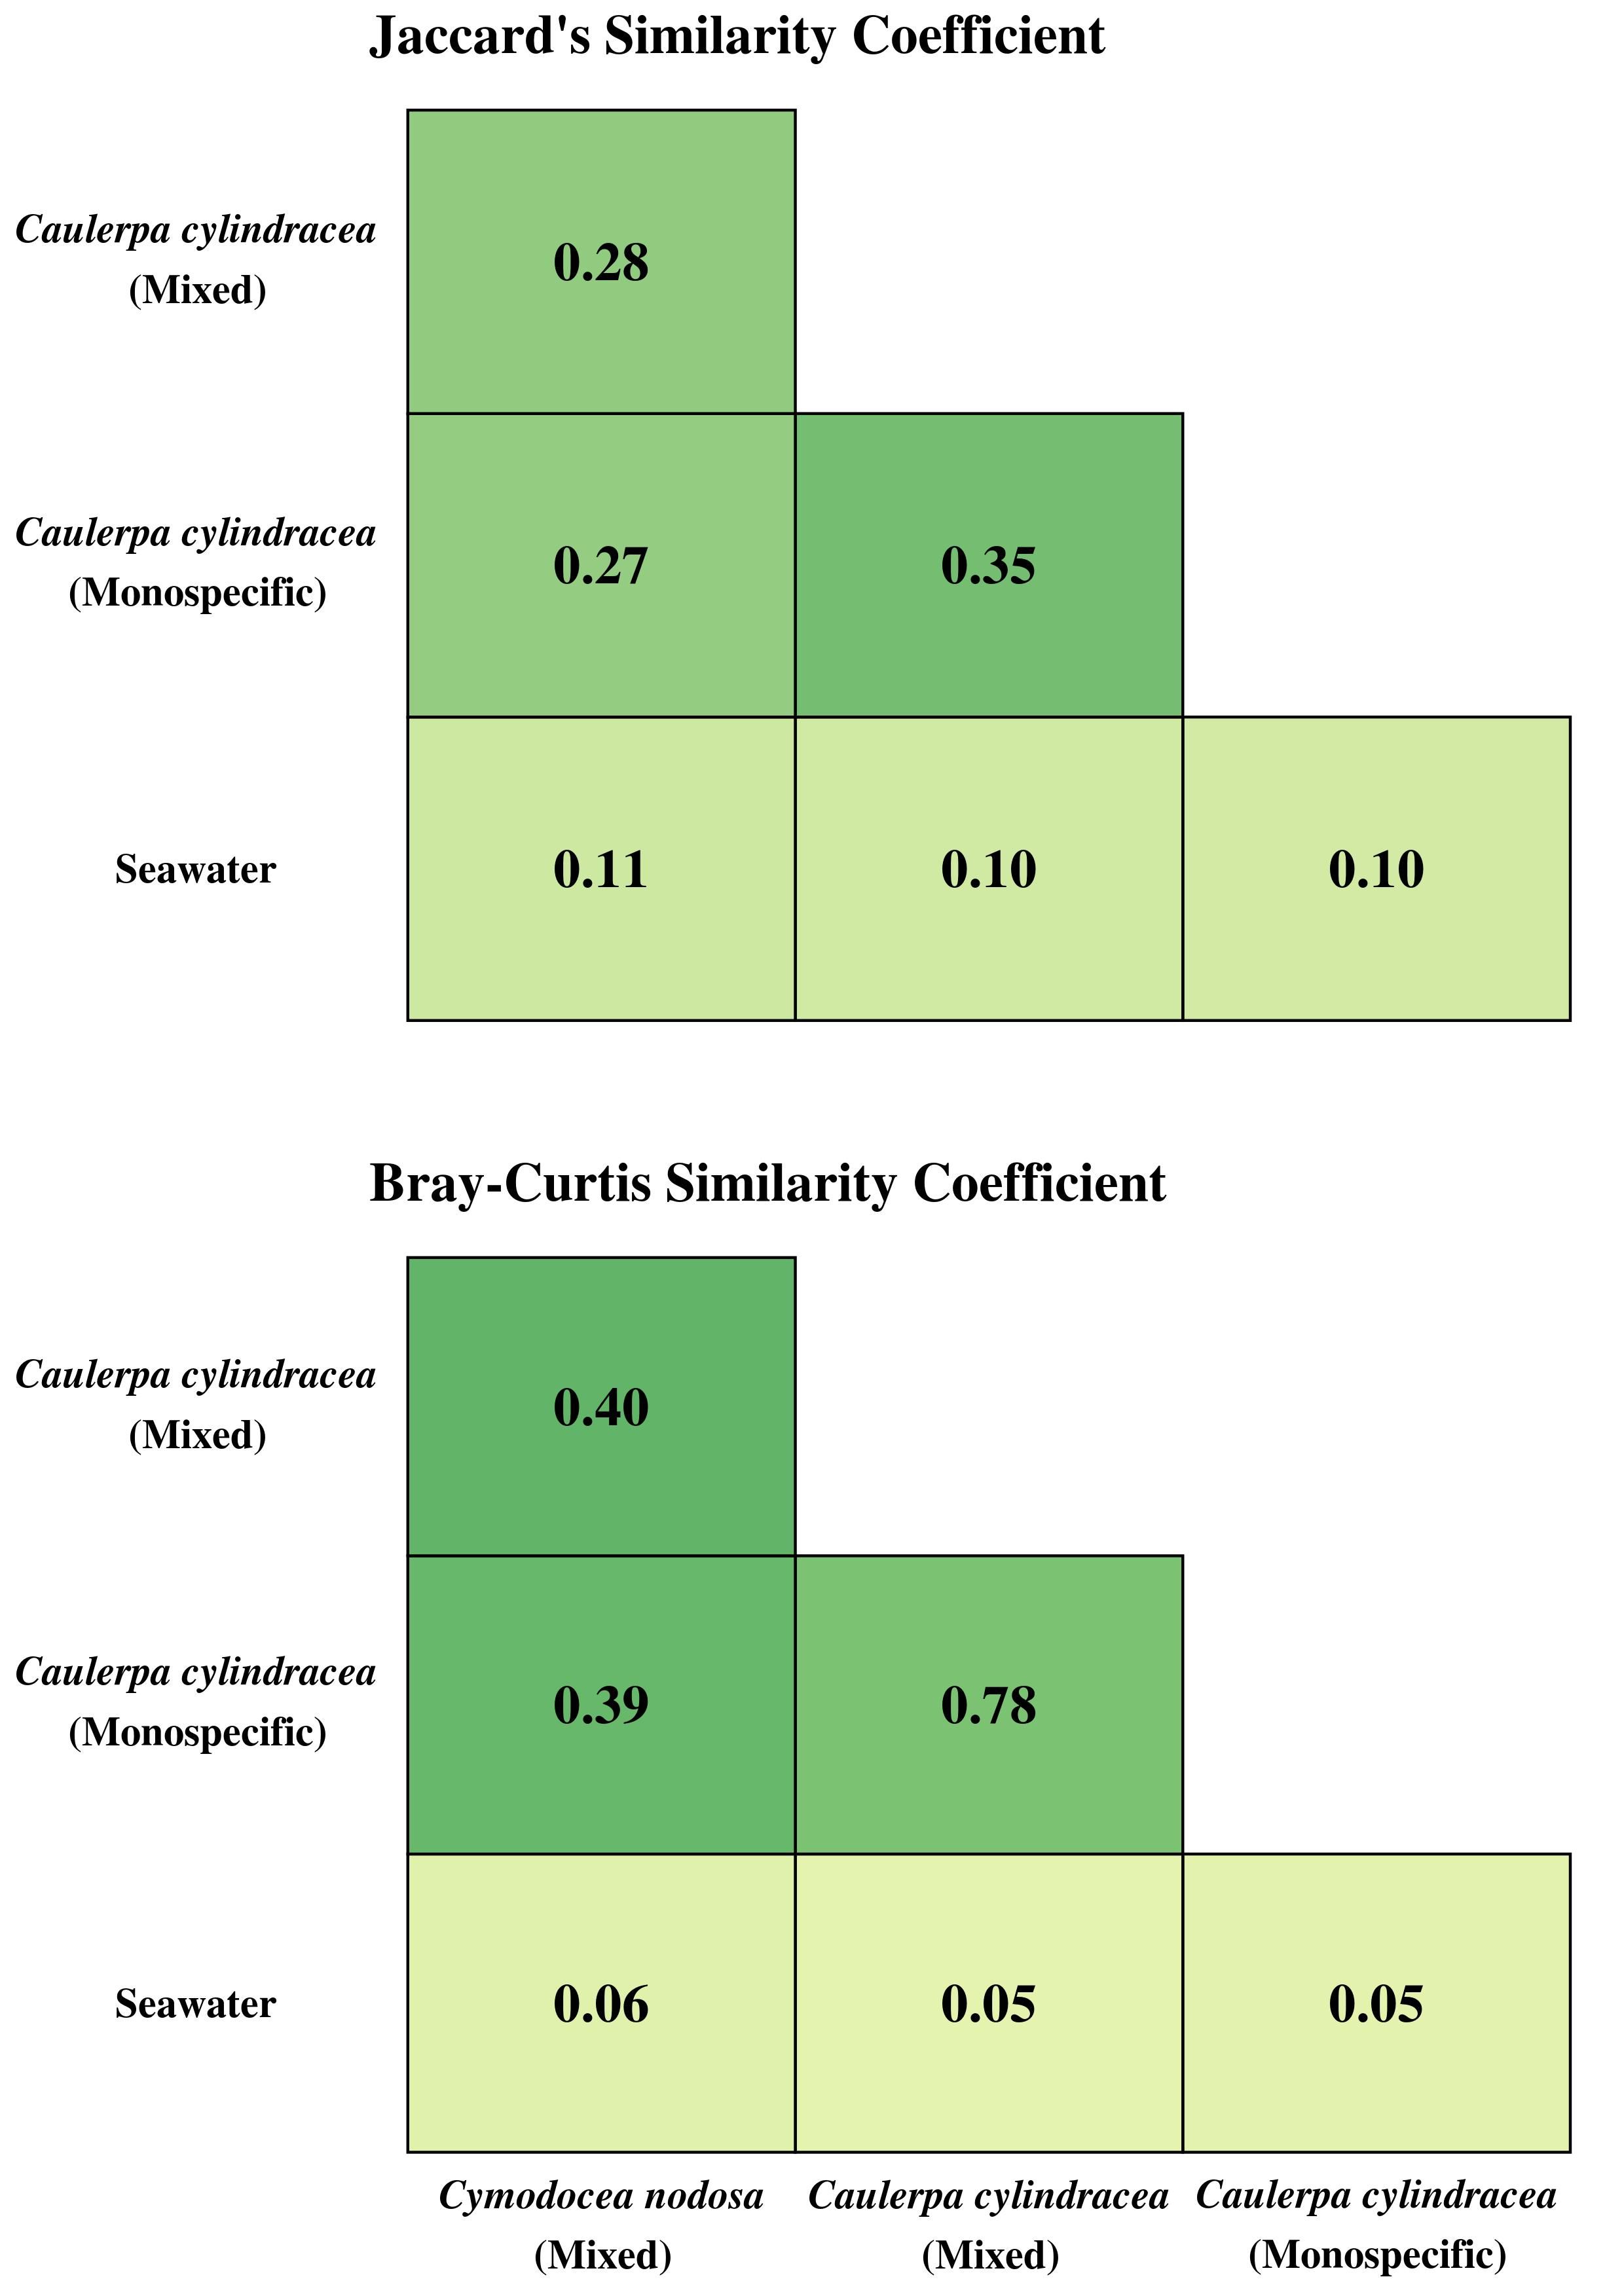
\includegraphics[width=0.7\linewidth]{../results/figures/matrix} 

}

\caption{Proportion of shared bacterial and archaeal OTUs (Jaccard's Similarity Coefficient) and shared bacterial and archaeal communities (Bray-Curtis Similarity Coefficient) between communties associated with the surfaces of macrophytes (\textit{Cymodocea nodosa} [Invaded] and \textit{Caulerpa cylindracea} [Invaded and Noninvaded]) and coomunities in the surrounding seawater.\label{matrix}}\label{fig:unnamed-chunk-1}
\end{figure}

\begin{figure}[H]

{\centering 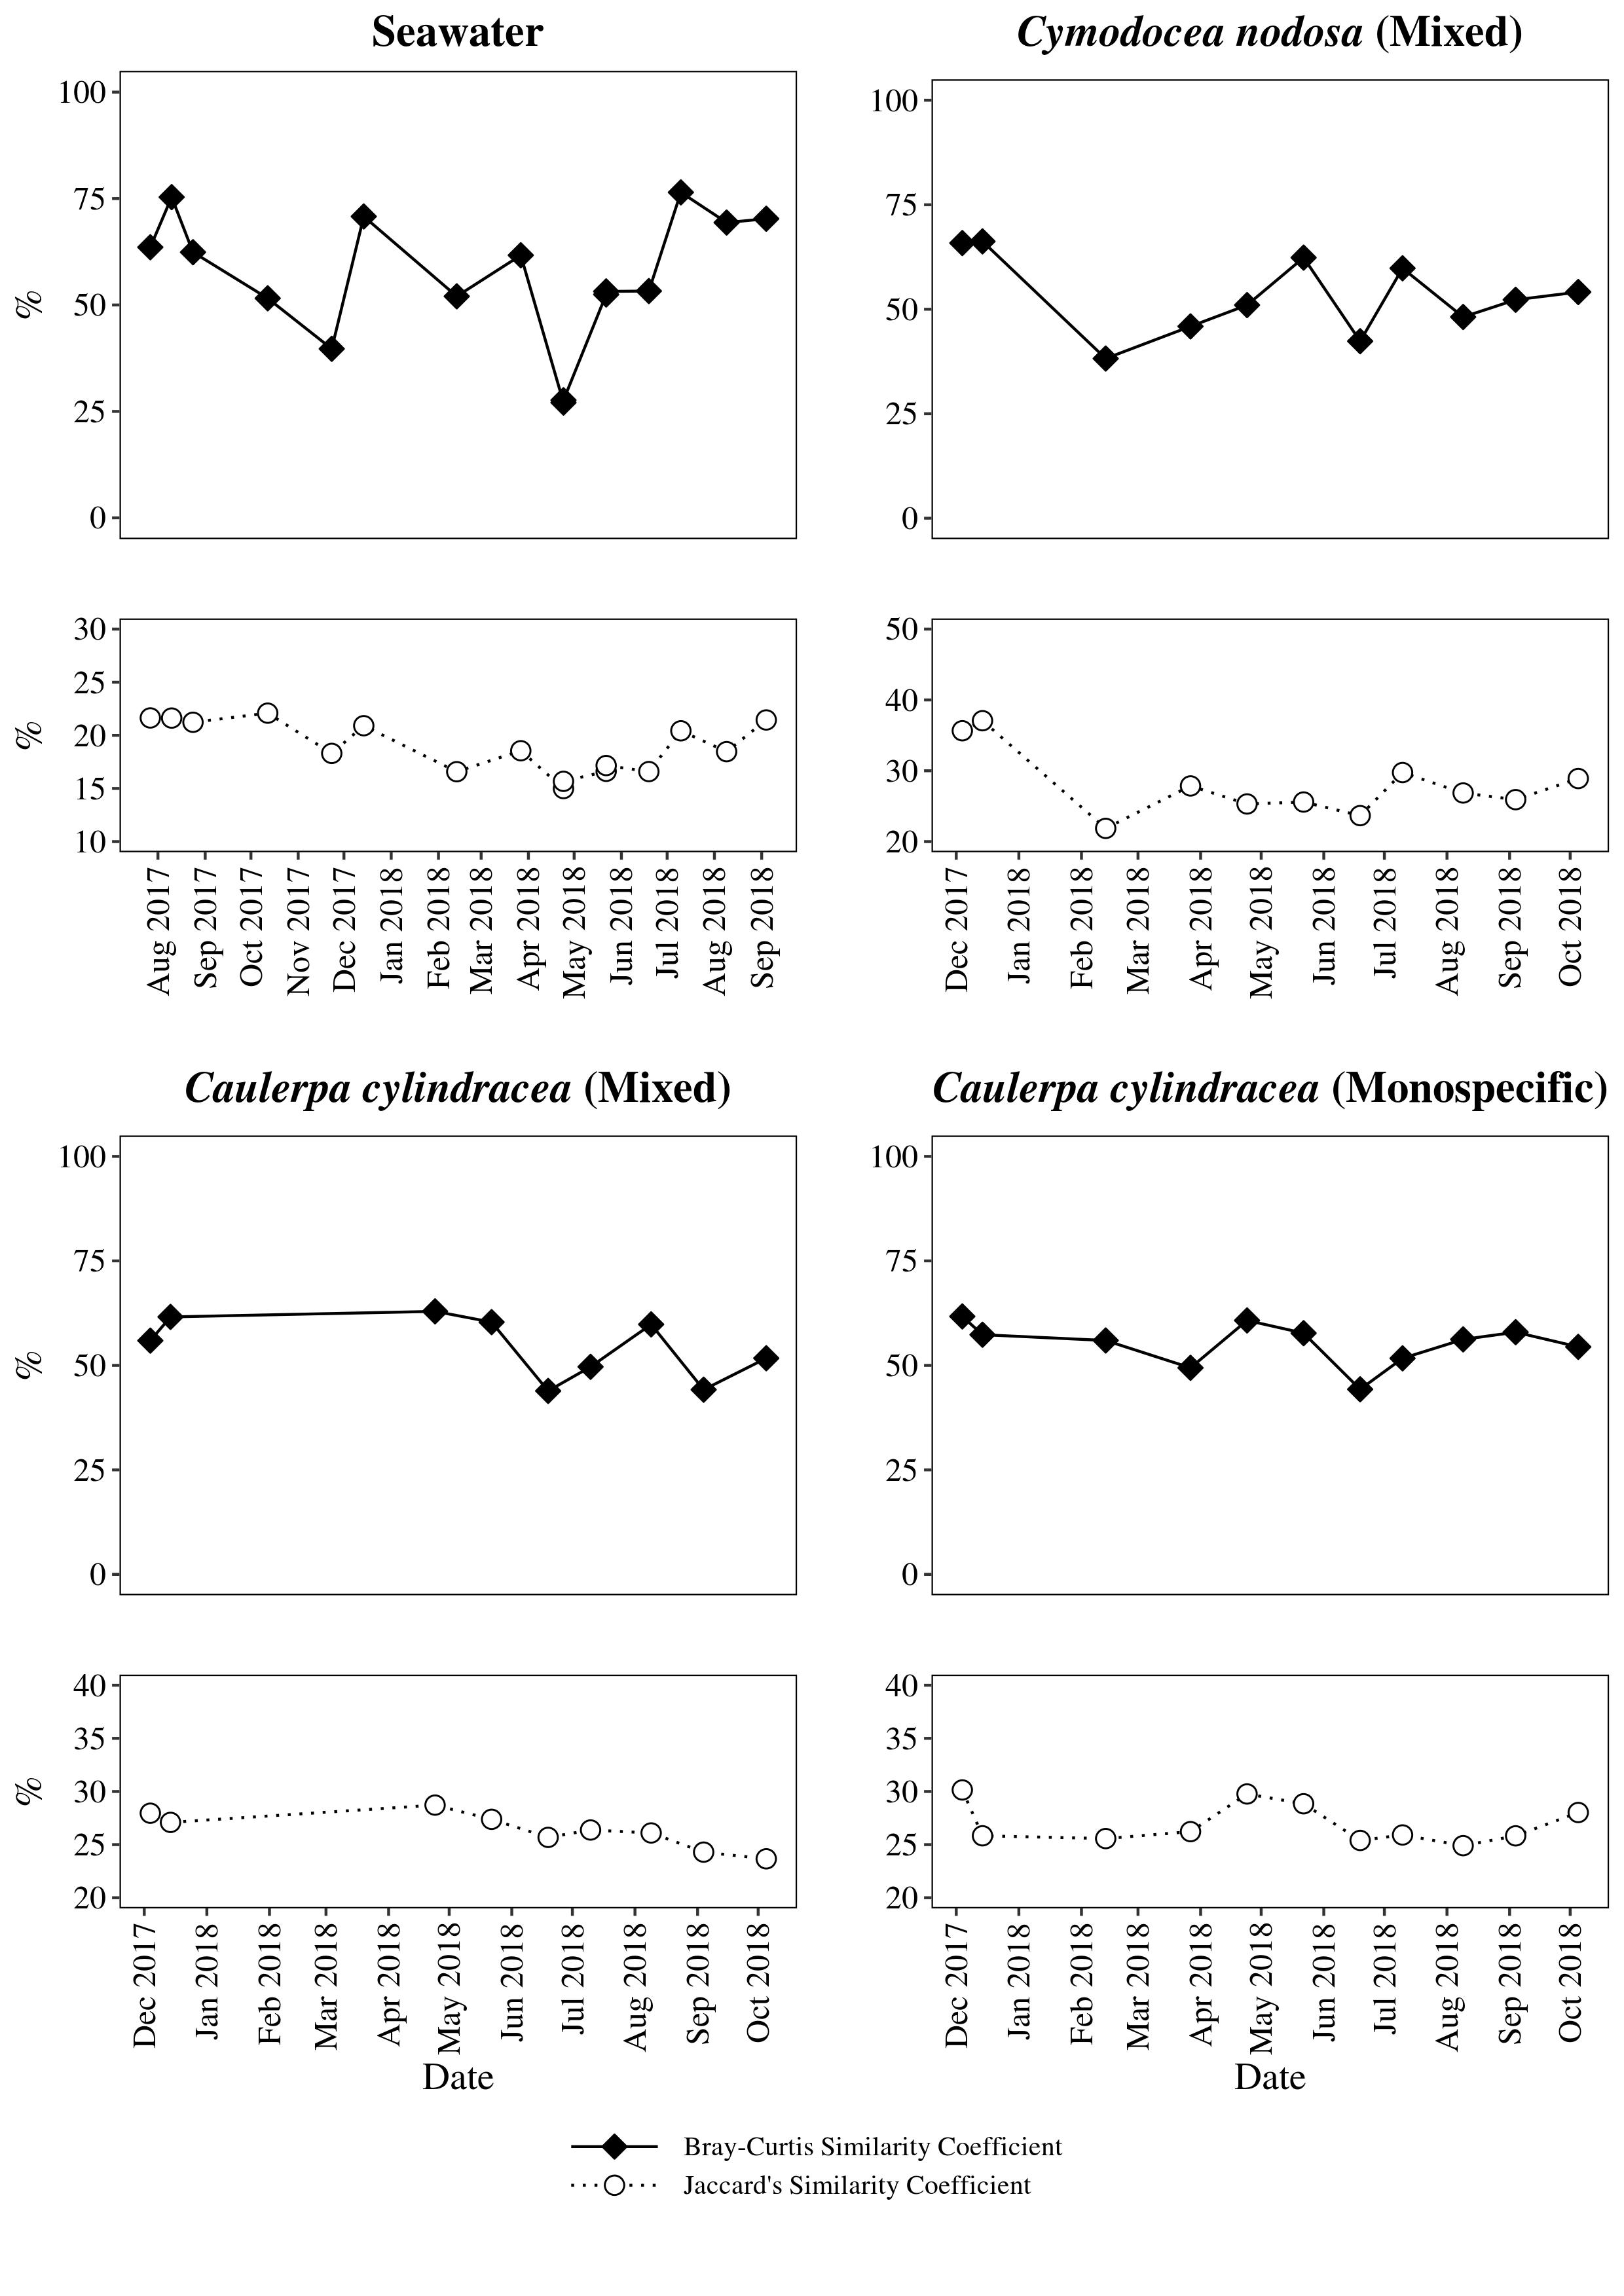
\includegraphics[width=0.85\linewidth]{../results/figures/seasonal_shared} 

}

\caption{Proprotion of shared bacterial and archaeal communities (Bray-Curtis Similarity Coefficient) and shared bacterial and archaeal OTUs (Jaccard's Similarity Coefficient) between consecutive sampling points and from the surfaces of macrophytes (\textit{Cymodocea nodosa} [Invaded] and \textit{Caulerpa cylindracea} [Invaded and Noninvaded]) and in the surrounding seawater.\label{shared}}\label{fig:unnamed-chunk-2}
\end{figure}

\begin{figure}[H]

{\centering 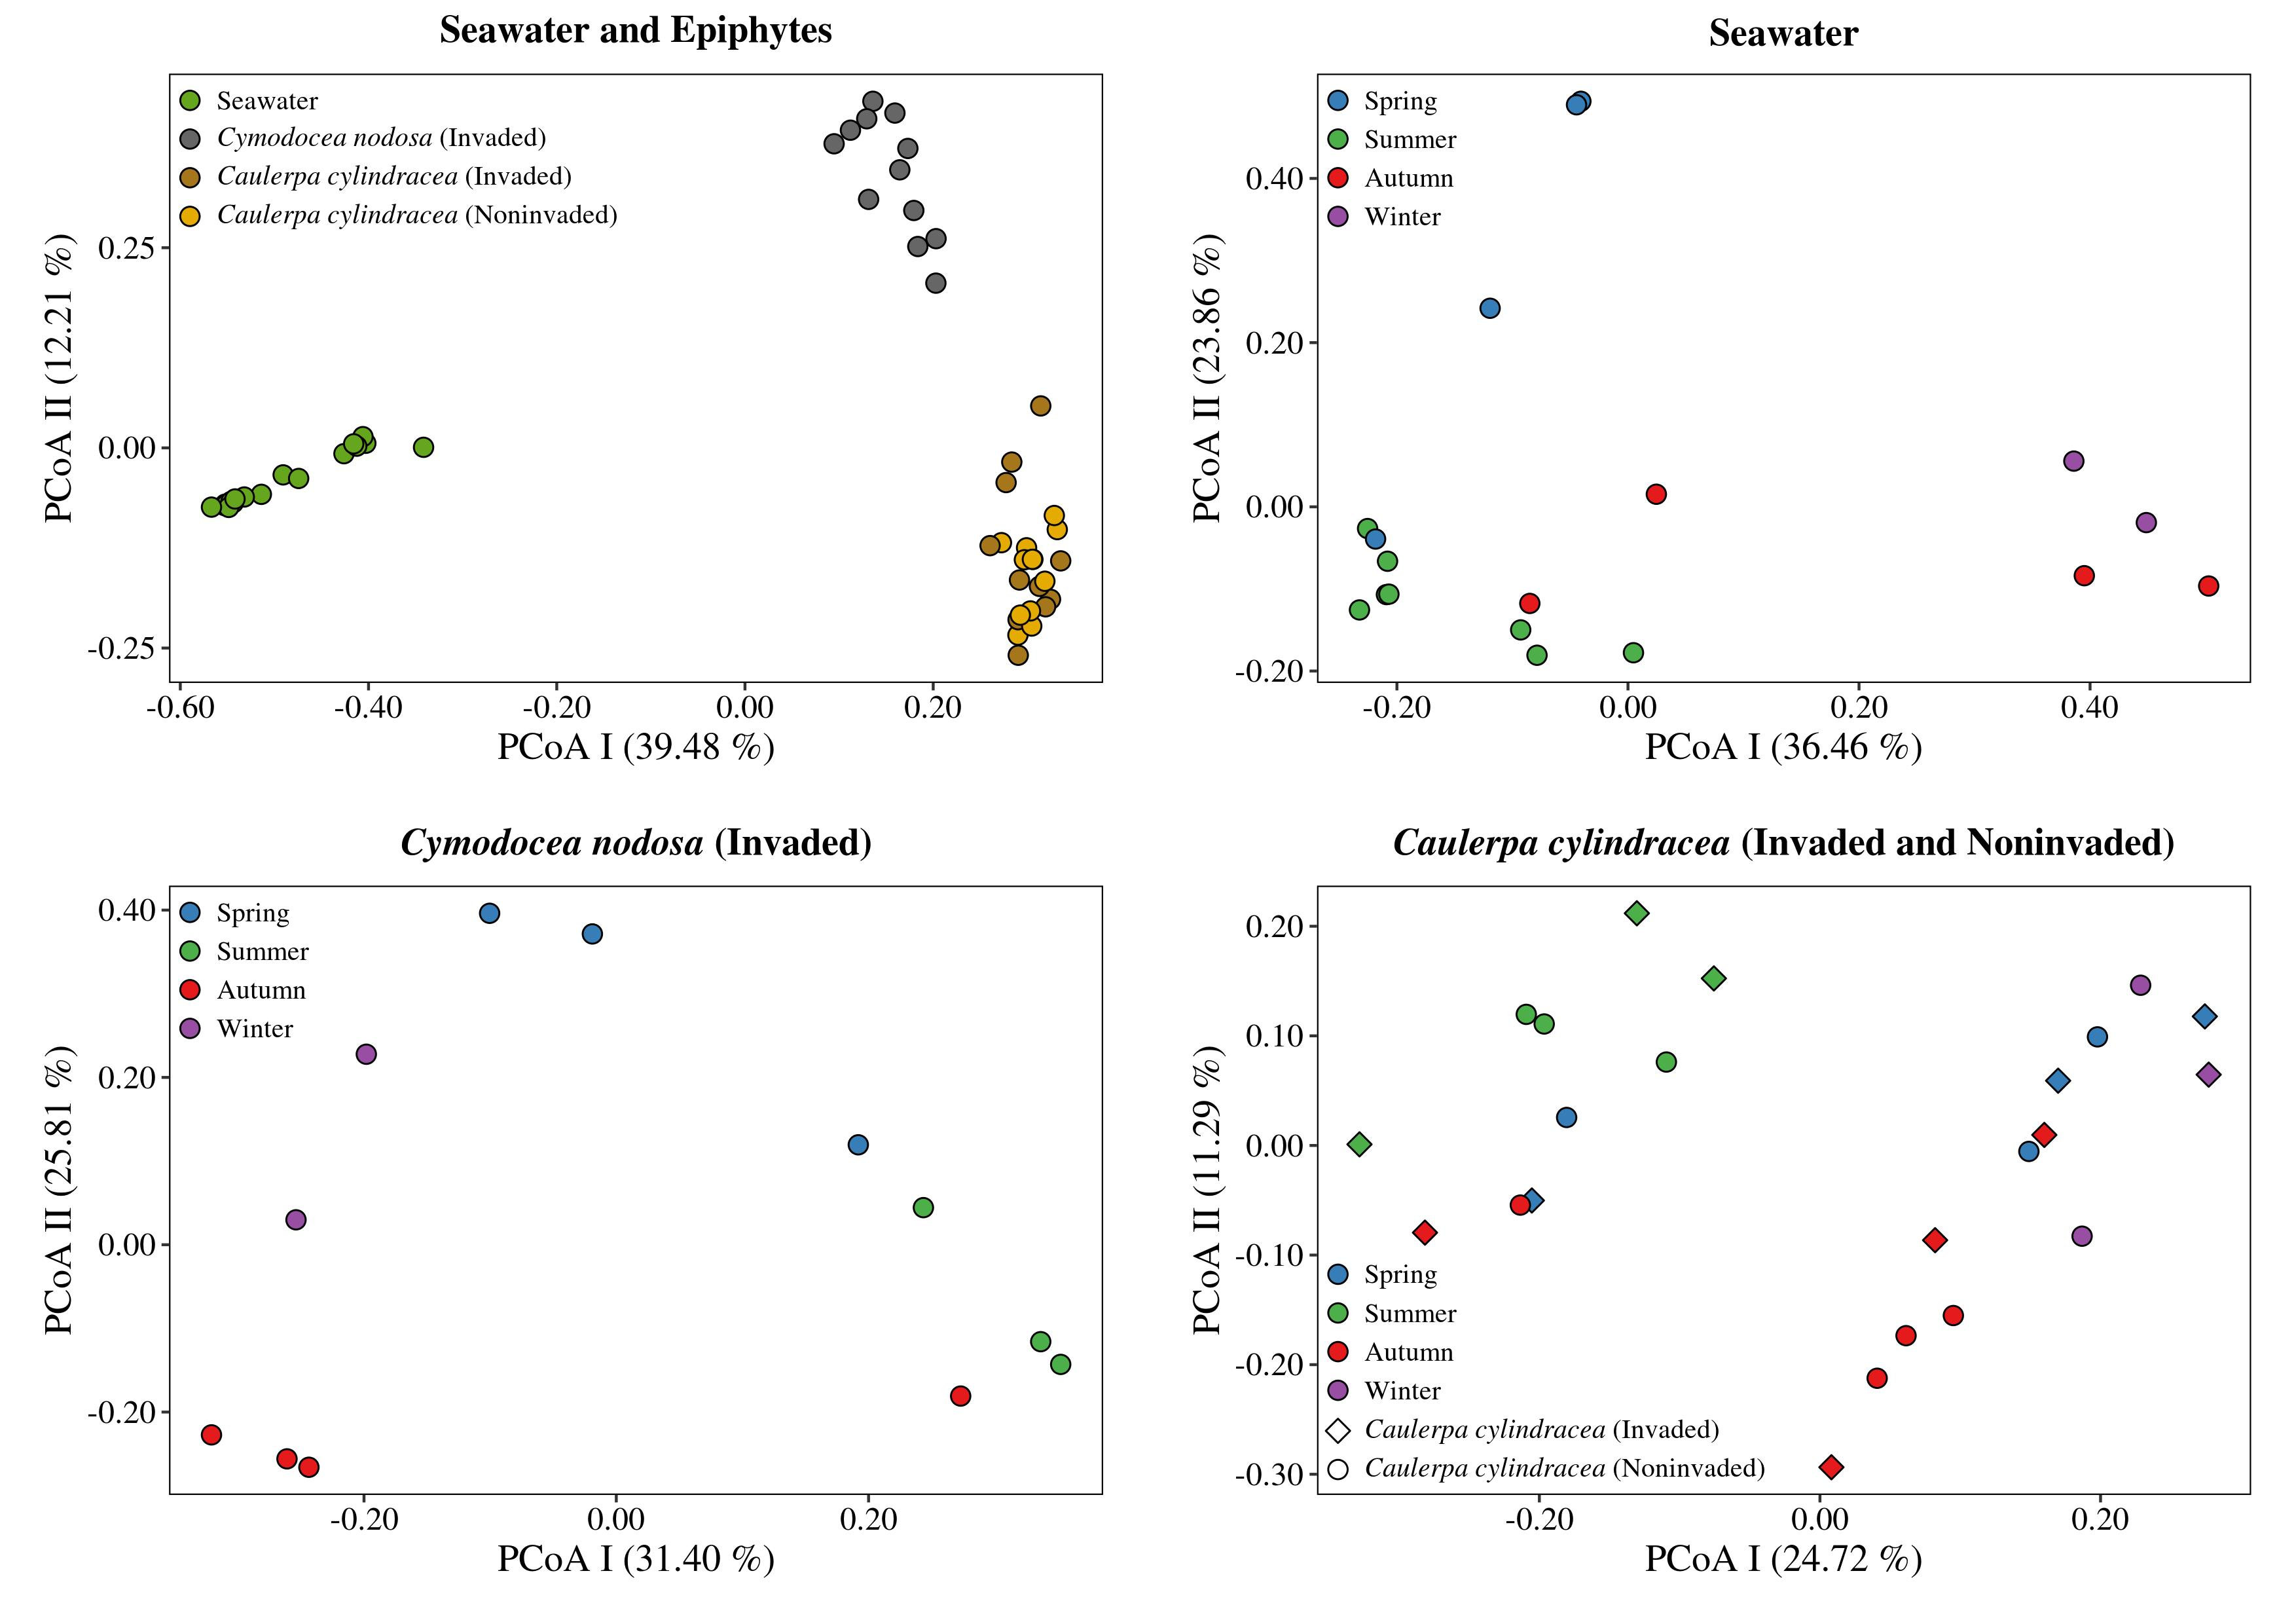
\includegraphics[width=1\linewidth]{../results/figures/pcoa_figure} 

}

\caption{Principal Coordinates Analysis (PCoA) of Bray-Curtis distances based on OTU abundances of bacterial and archaeal communities from the surfaces of macrophytes (\textit{Cymodocea nodosa} [Invaded] and \textit{Caulerpa cylindracea} [Invaded and Noninvaded]) and in the surrounding seawater. Samples from the same environment or same season are labeld in different colors. The proportion of explained variation by each axis is shown on the corresponding axis in parentheses.\label{pcoa}}\label{fig:unnamed-chunk-3}
\end{figure}

\begin{figure}[H]

{\centering 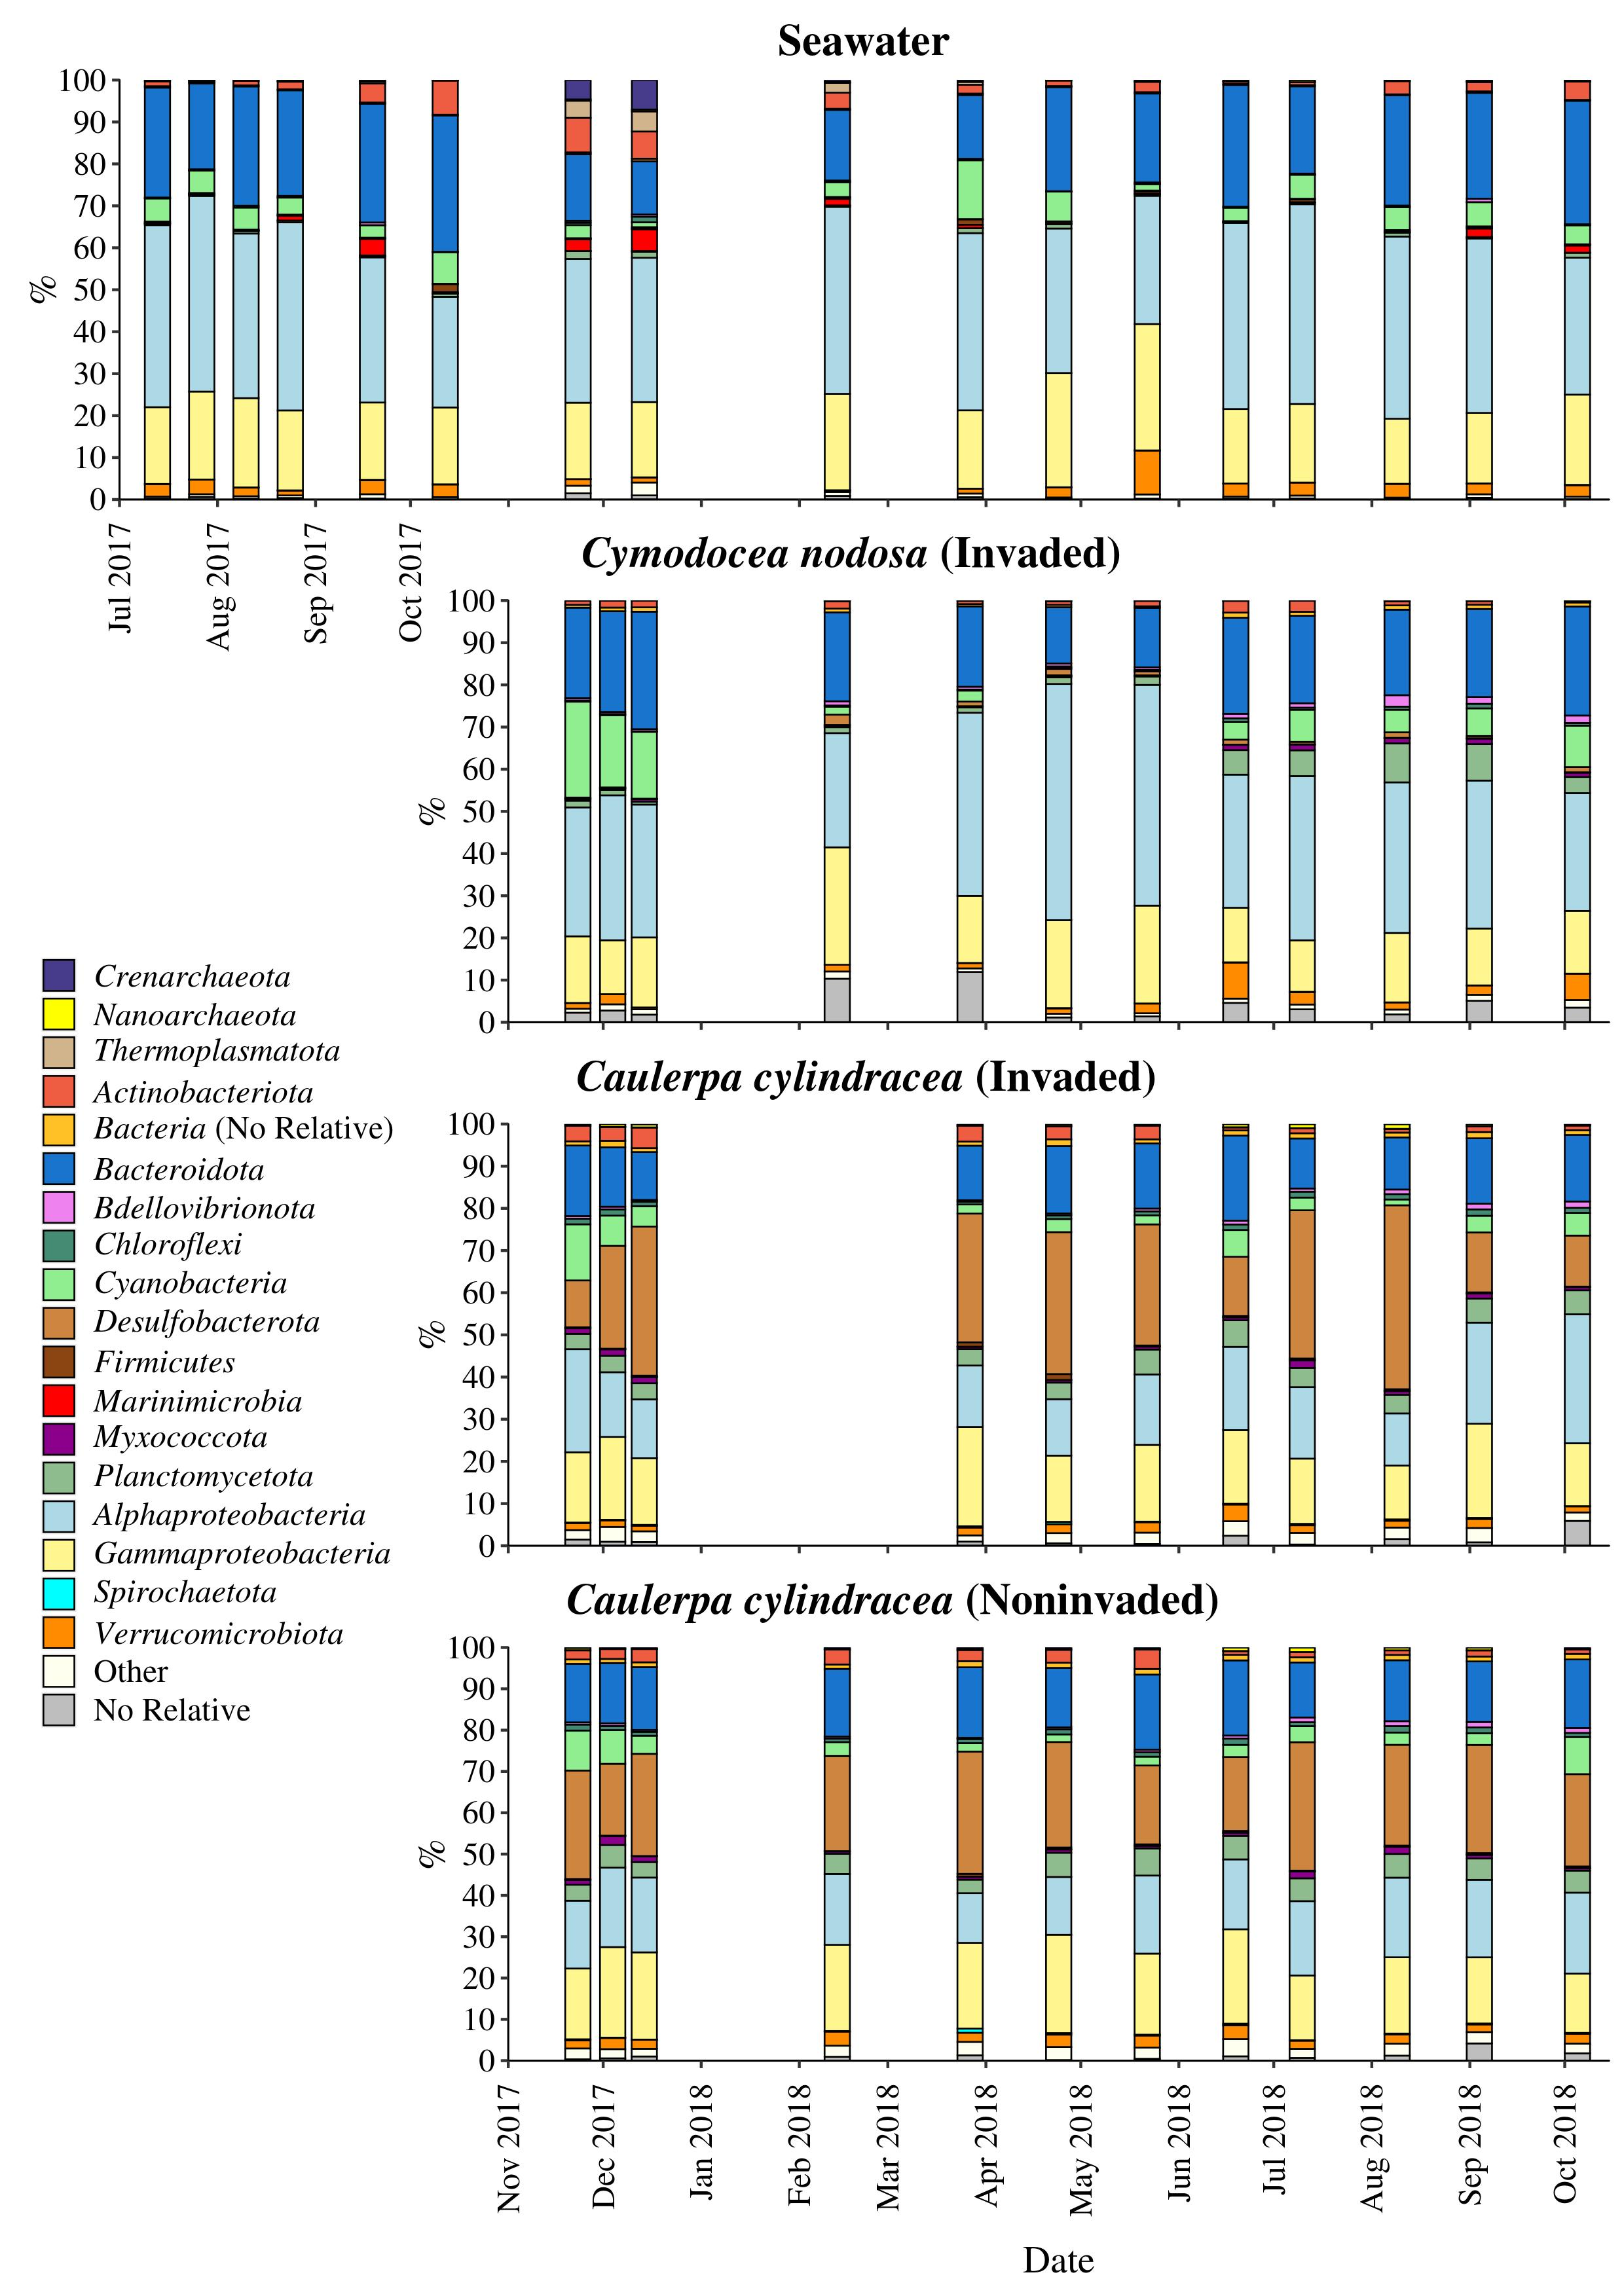
\includegraphics[width=0.85\linewidth]{../results/figures/community_bar_plot} 

}

\caption{Taxonomic classification and relative contribution of the most abundant bacterial and archaeal sequences on the surfaces of macrophytes (\textit{Cymodocea nodosa} [Invaded] and \textit{Caulerpa cylindracea} [Invaded and Noninvaded]) and in the surrounding seawater.\label{community}}\label{fig:unnamed-chunk-4}
\end{figure}

\begin{figure}[H]

{\centering 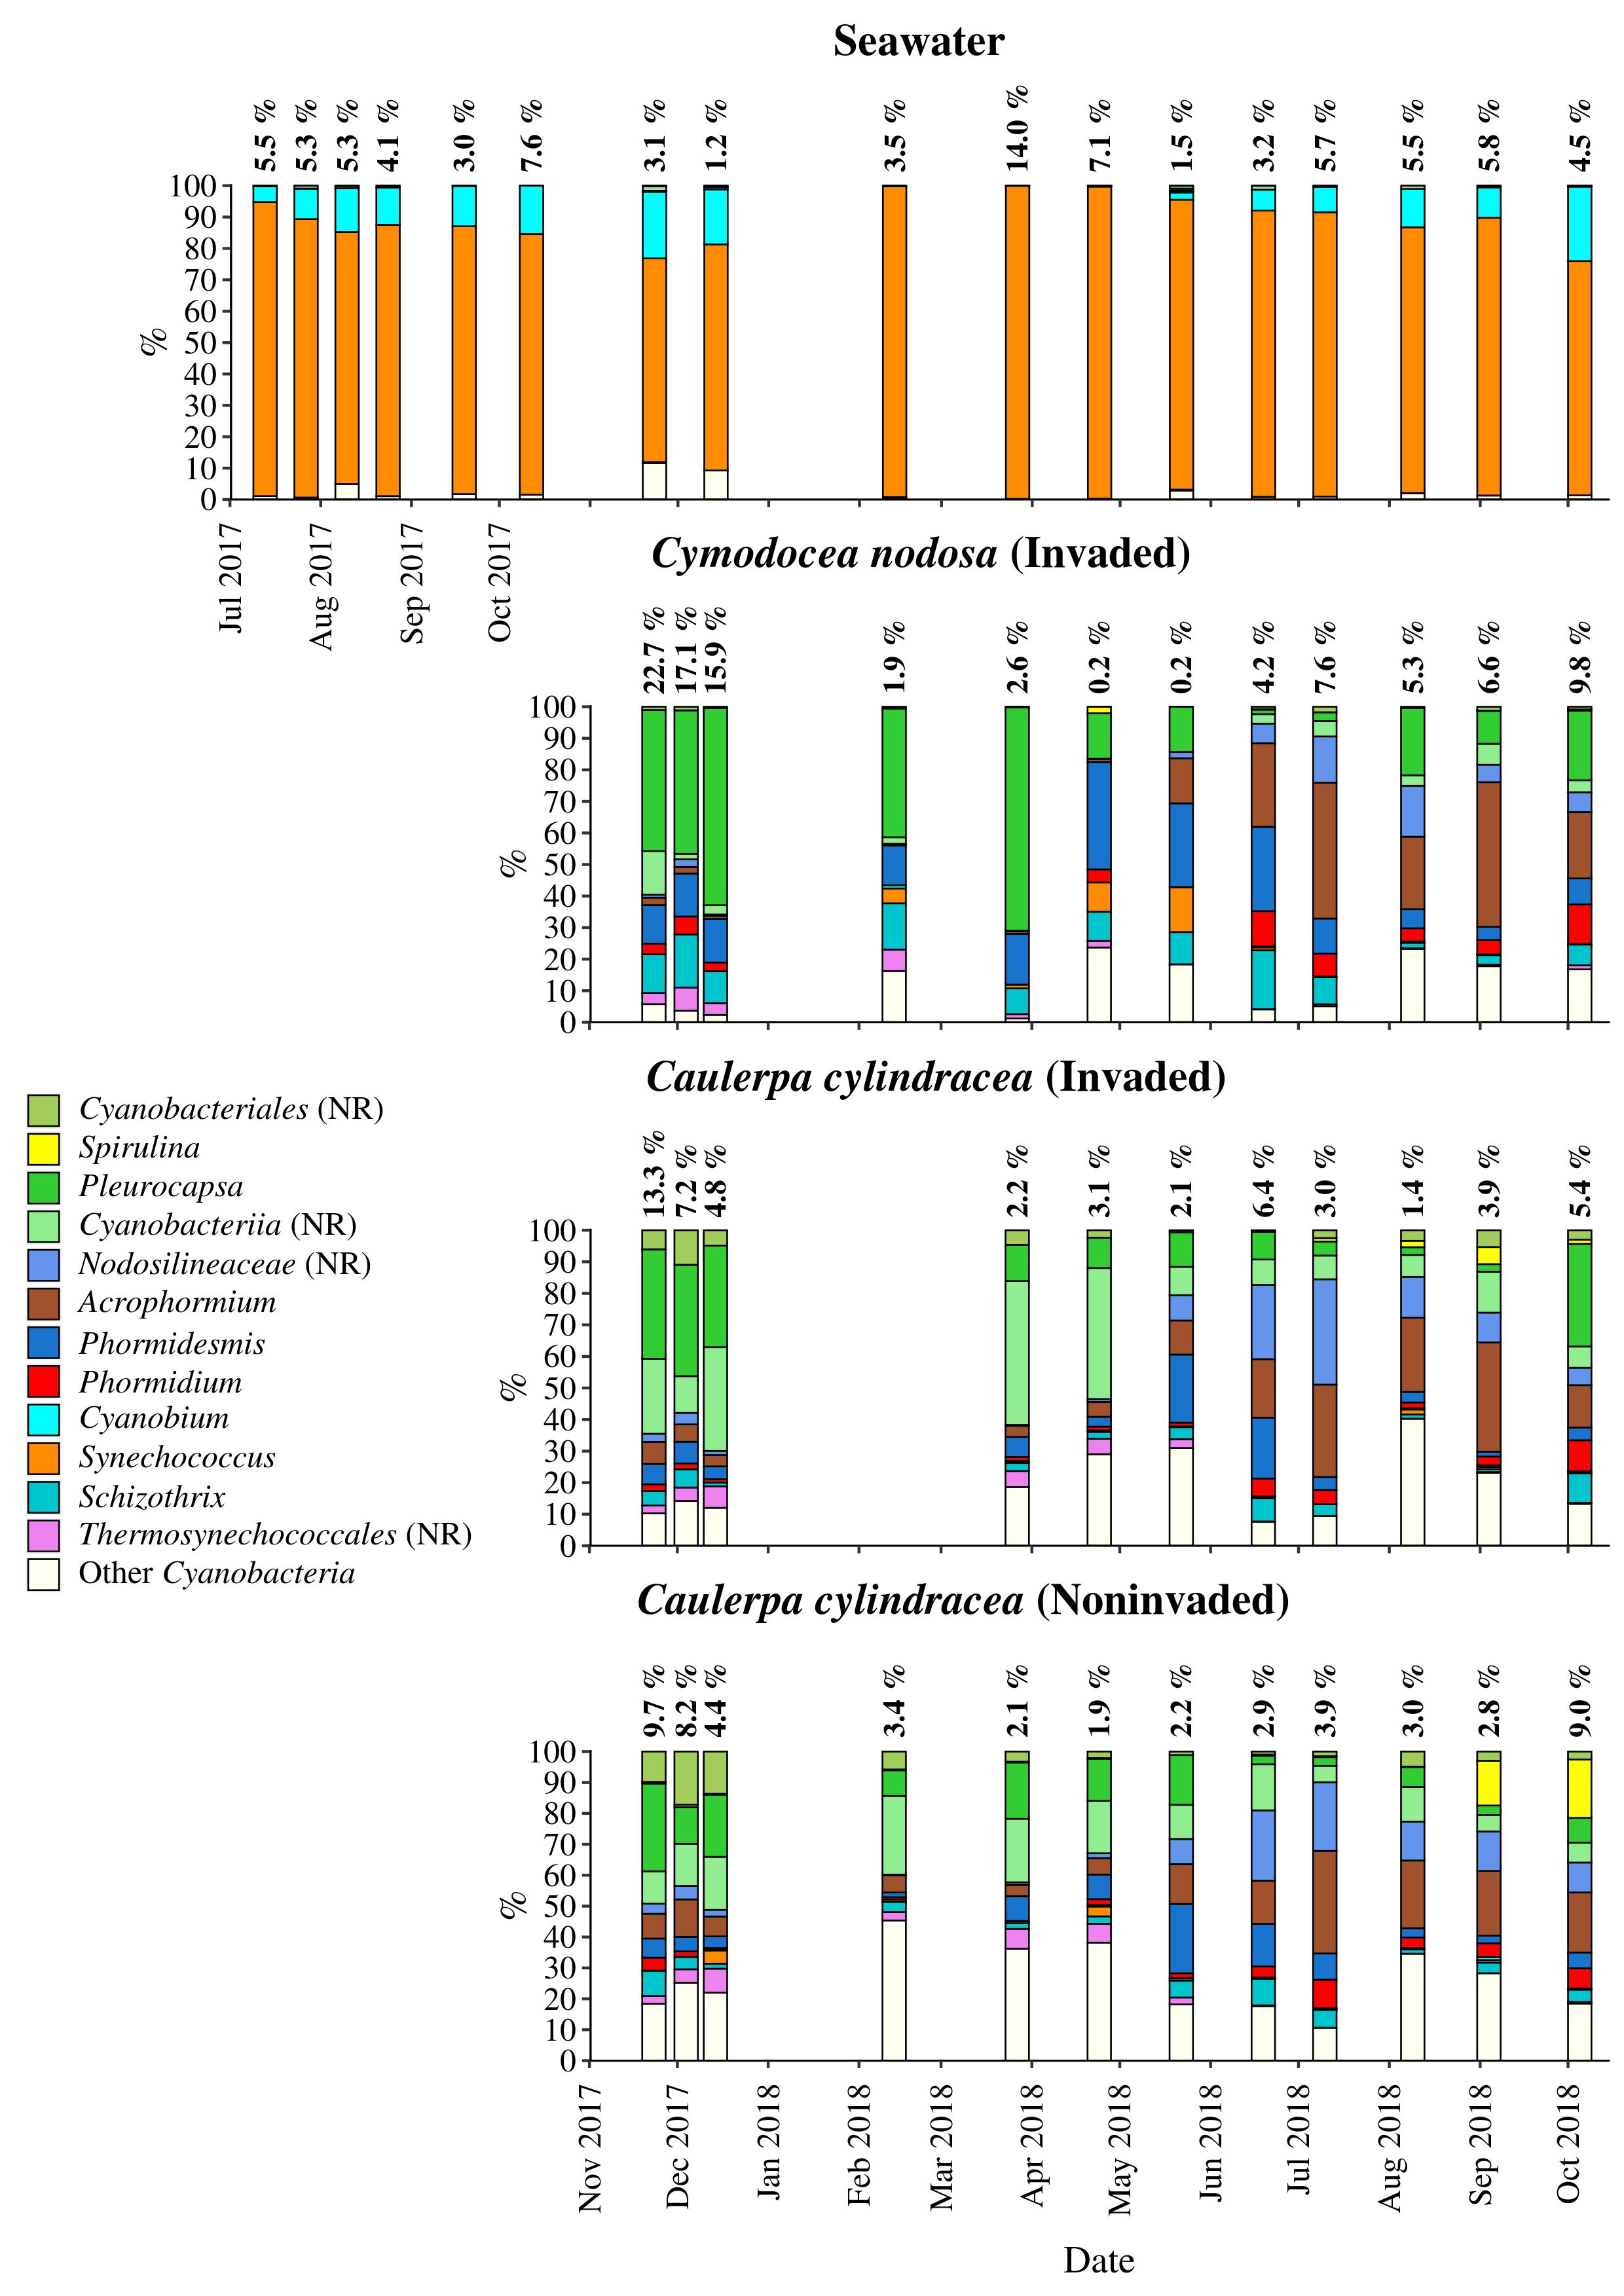
\includegraphics[width=0.85\linewidth]{../results/figures/cyanobacteria_bar_plot} 

}

\caption{Taxonomic classification and relative contribution of the most abundant cyanobacterial sequences on the surfaces of macrophytes (\textit{Cymodocea nodosa} [Invaded] and \textit{Caulerpa cylindracea} [Invaded and Noninvaded]) and in the surrounding seawater. The proprotion of cyanobaterial sequences in the total bacterial and archaeal community is given above the corresponding bar. NR -- No Relative\label{cyano}}\label{fig:unnamed-chunk-5}
\end{figure}

\begin{figure}[H]

{\centering 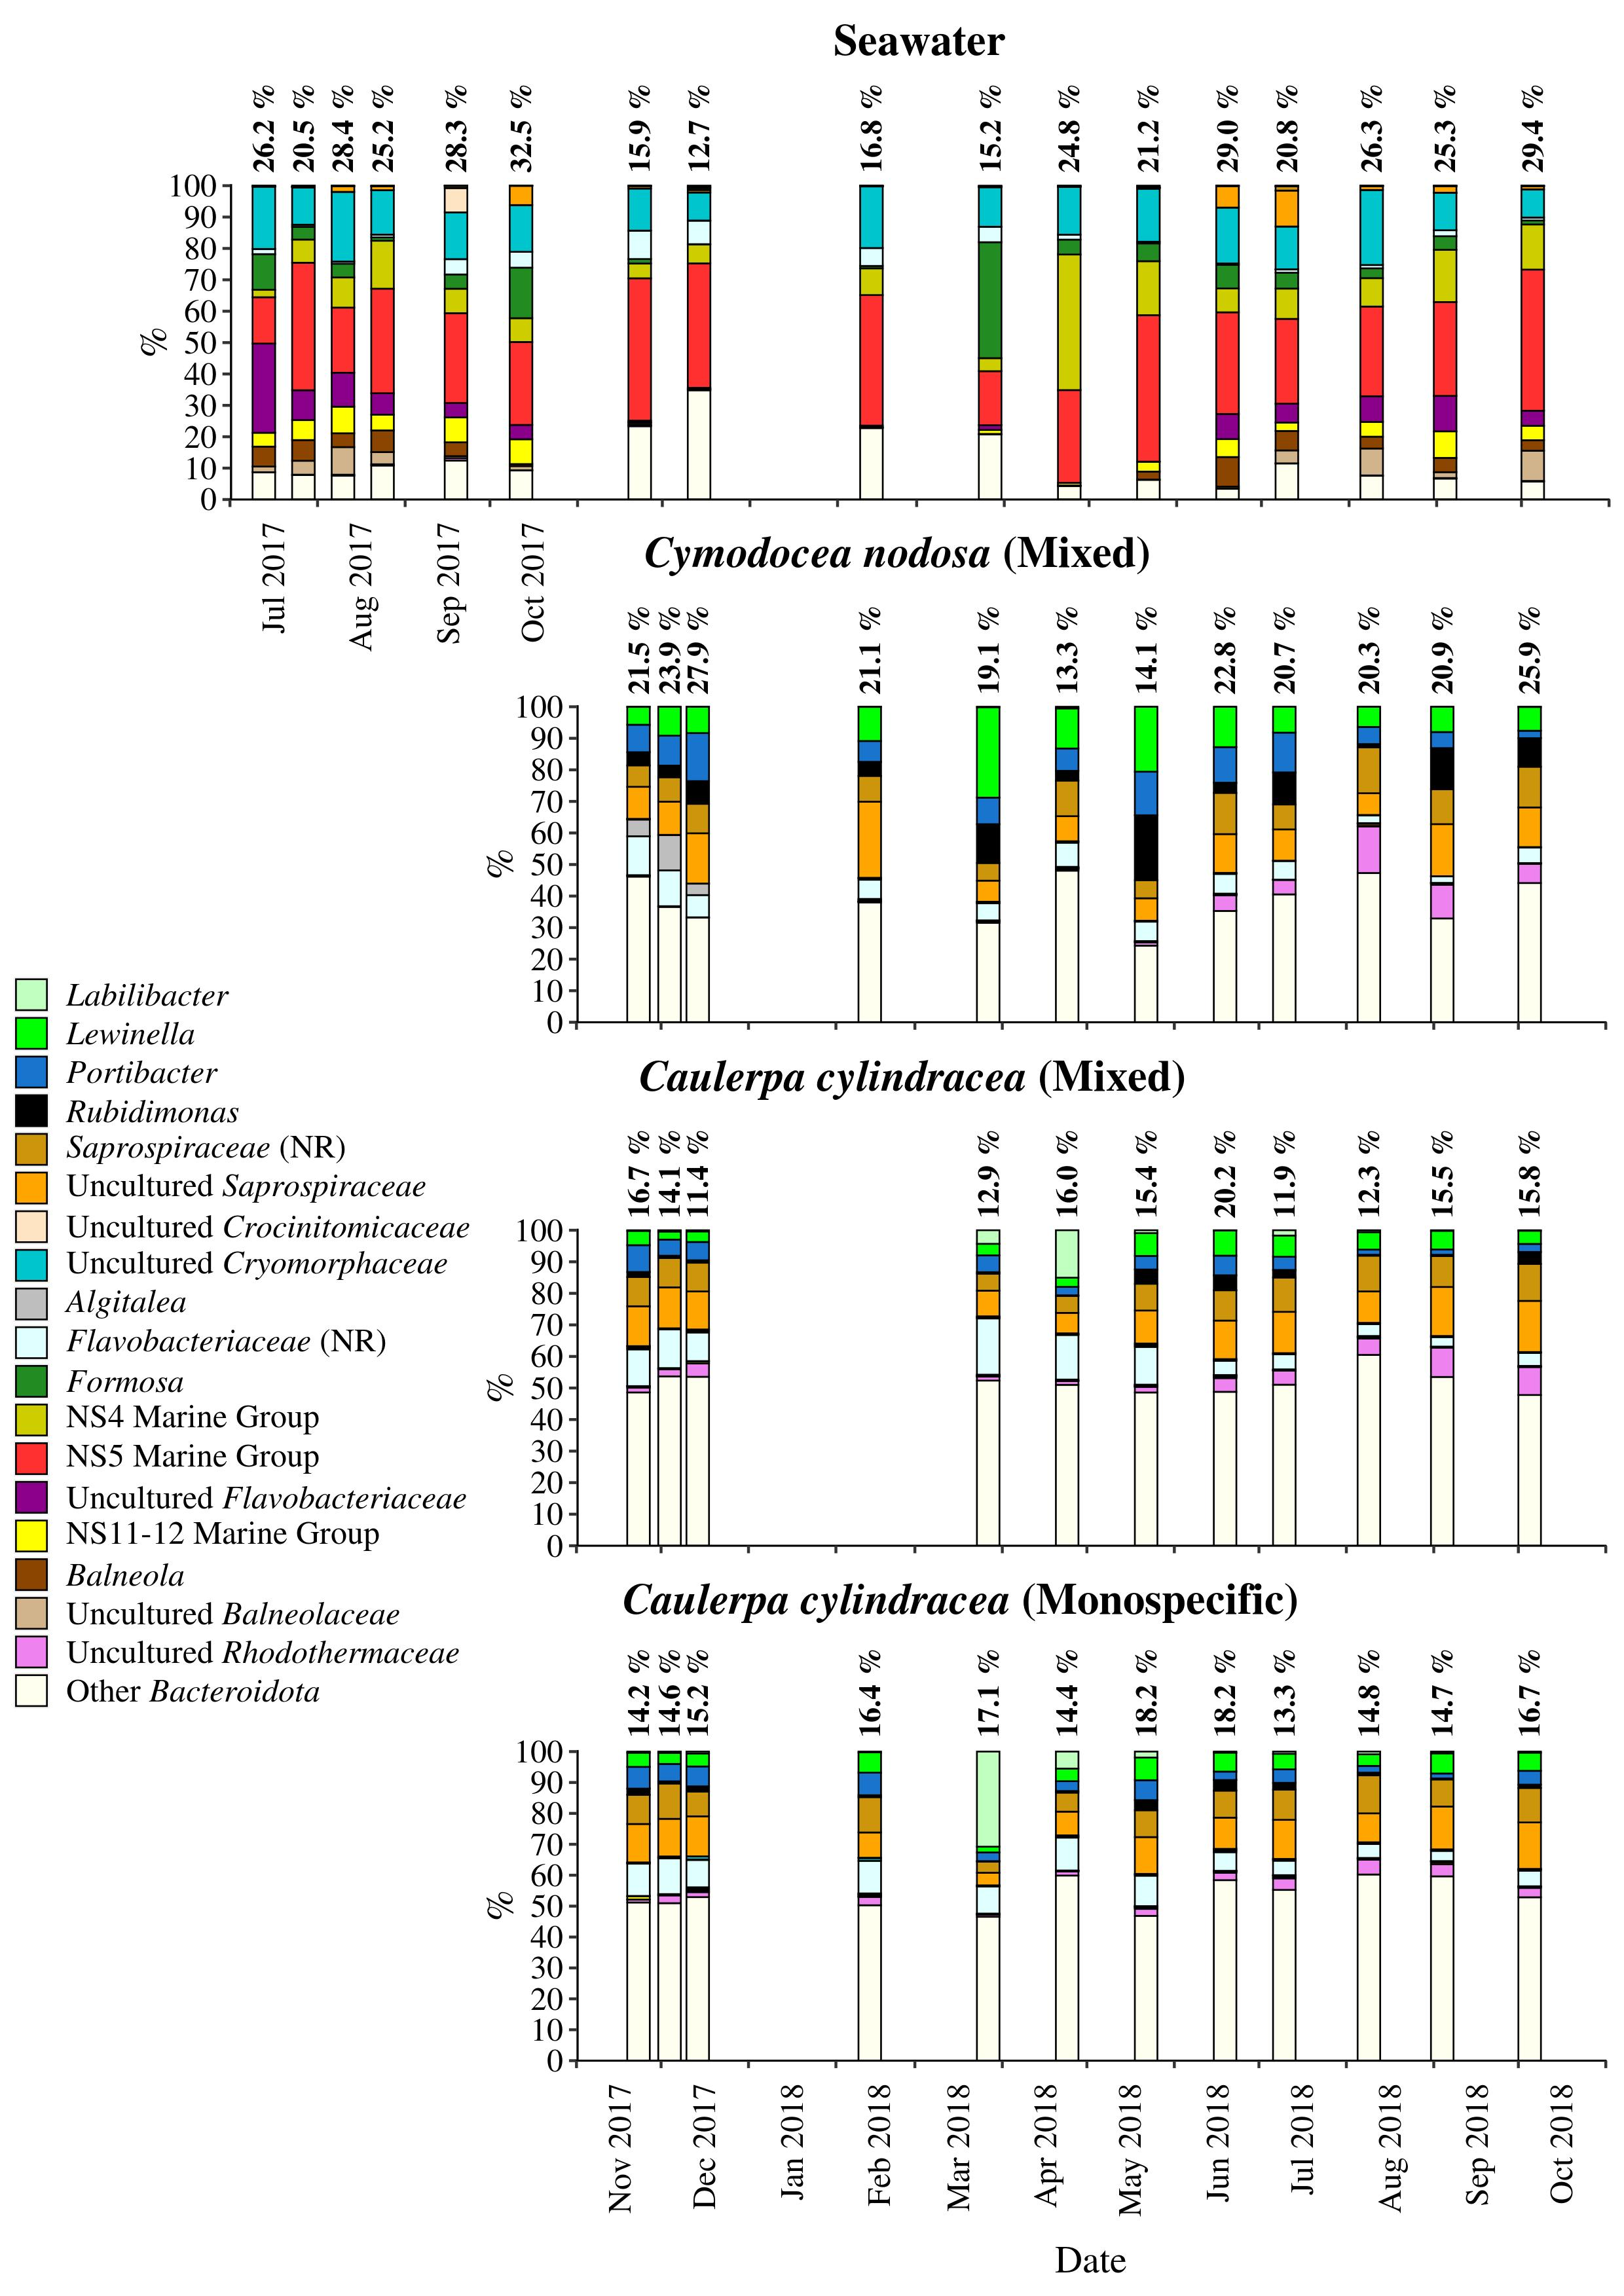
\includegraphics[width=0.85\linewidth]{../results/figures/bacteroidota_bar_plot} 

}

\caption{Taxonomic classification and relative contribution of the most abundant sequences within the \textit{Bacteroidota} on the surfaces of macrophytes (\textit{Cymodocea nodosa} [Invaded] and \textit{Caulerpa cylindracea} [Invaded and Noninvaded]) and in the surrounding seawater. The proprotion of sequences classified as \textit{Bacteroidota} in the total bacterial and archaeal community is given above the corresponding bar. NR -- No Relative\label{bactero}}\label{fig:unnamed-chunk-6}
\end{figure}

\begin{figure}[H]

{\centering 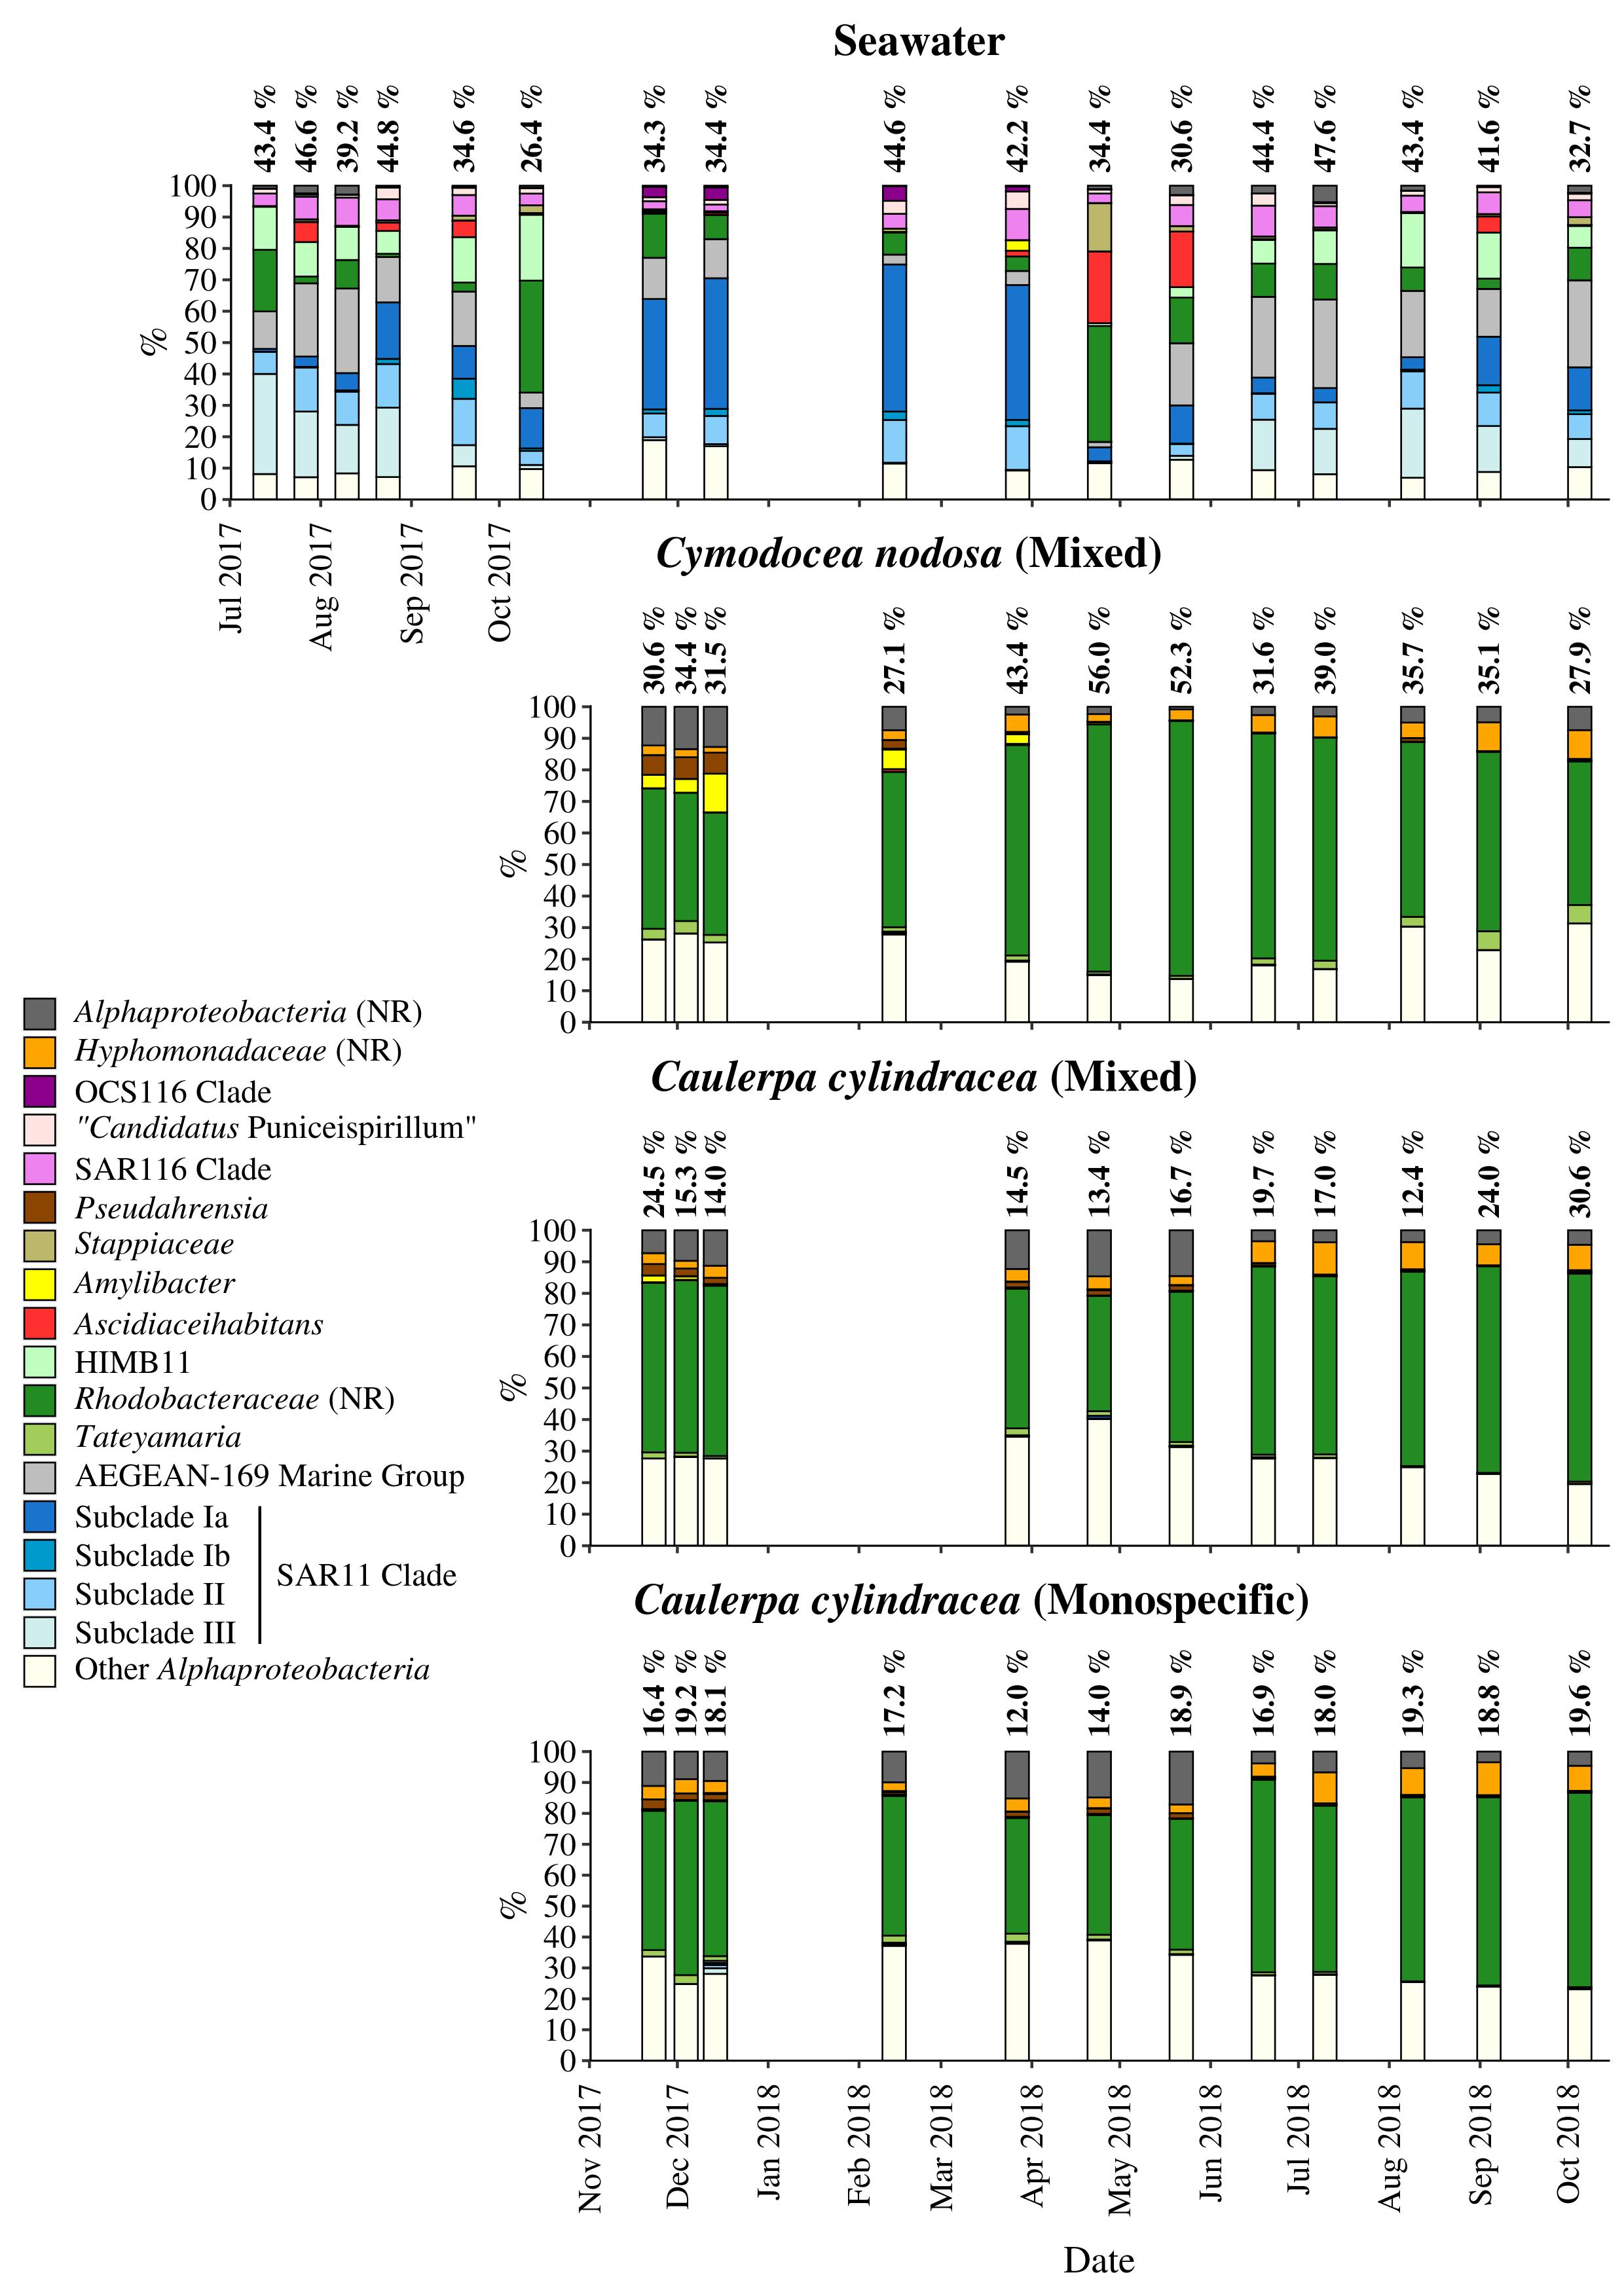
\includegraphics[width=0.85\linewidth]{../results/figures/alphaproteobacteria_bar_plot} 

}

\caption{Taxonomic classification and relative contribution of the most abundant alphaproteobacterial sequences on the surfaces of macrophytes (\textit{Cymodocea nodosa} [Invaded] and \textit{Caulerpa cylindracea} [Invaded and Noninvaded]) and in the surrounding seawater. The proprotion of alphaproteobacterial sequences in the total bacterial and archaeal community is given above the corresponding bar. NR -- No Relative\label{alpha}}\label{fig:unnamed-chunk-7}
\end{figure}

\begin{figure}[H]

{\centering 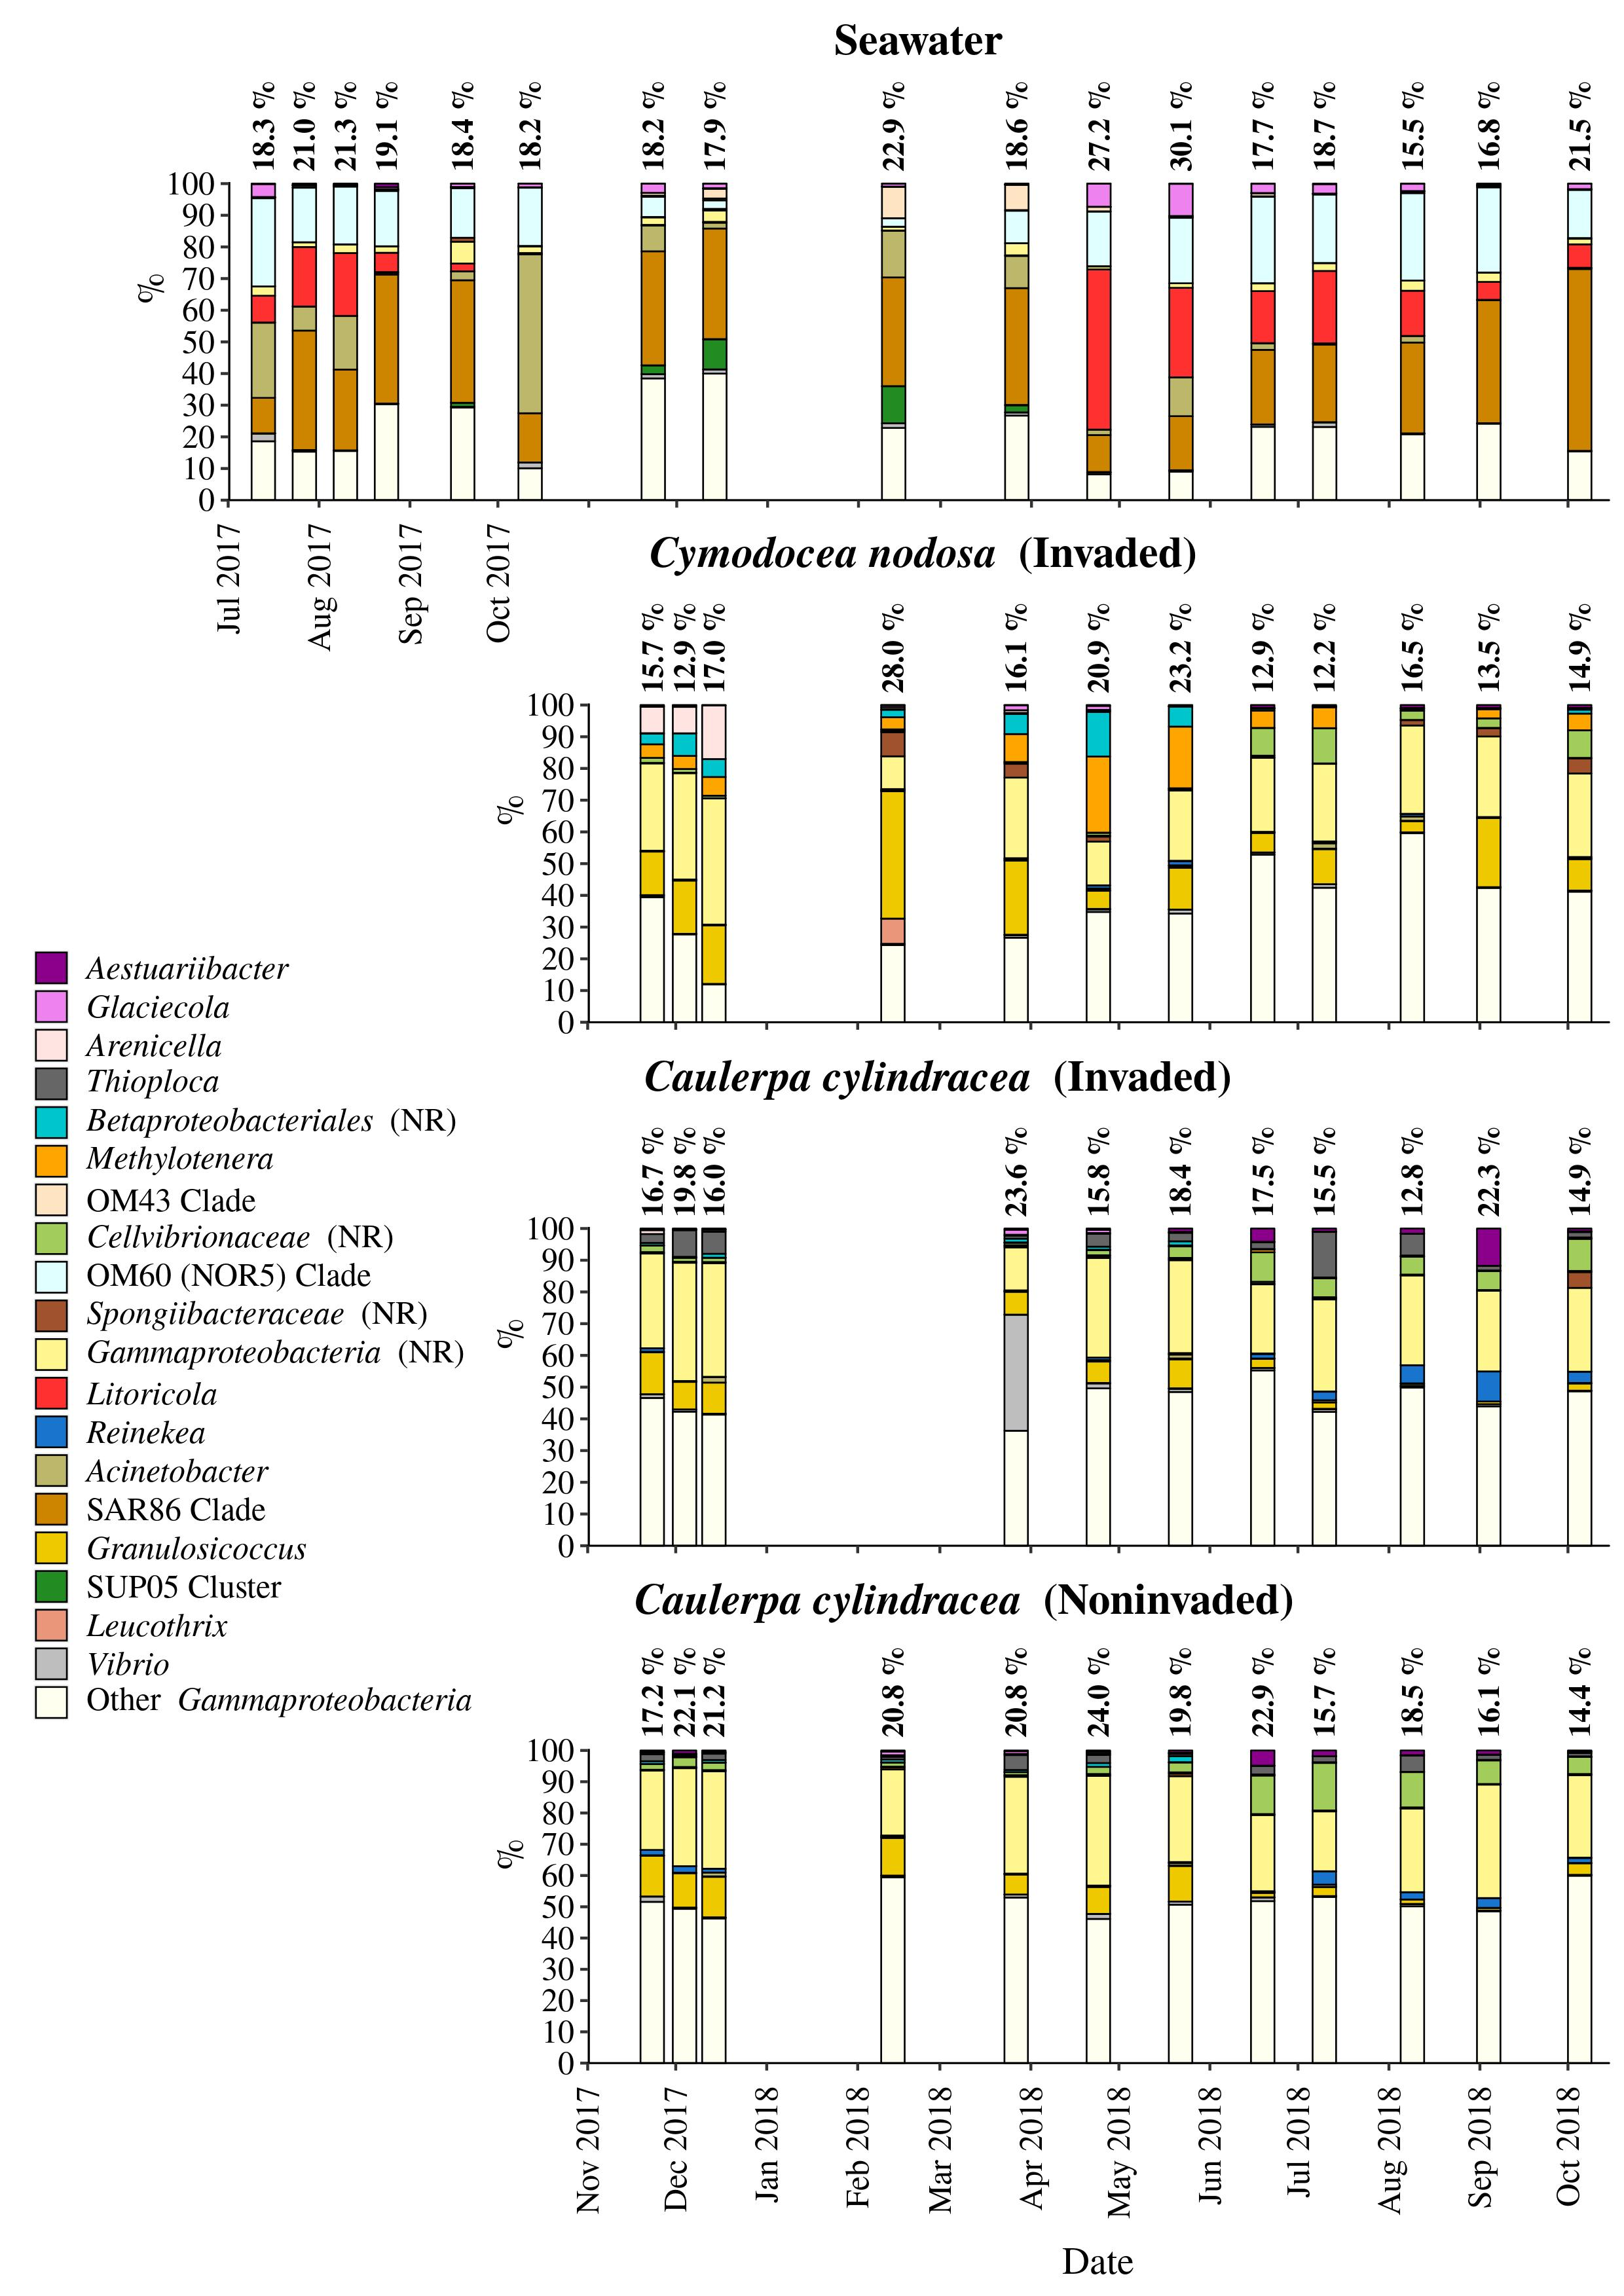
\includegraphics[width=0.85\linewidth]{../results/figures/gammaproteobacteria_bar_plot} 

}

\caption{Taxonomic classification and relative contribution of the most abundant gammaproteobacterial sequences on the surfaces of macrophytes (\textit{Cymodocea nodosa} [Invaded] and \textit{Caulerpa cylindracea} [Invaded and Noninvaded]) and in the surrounding seawater. The proprotion of gammaproteobacterial sequences in the total bacterial and archaeal community is given above the corresponding bar. NR -- No Relative\label{gamma}}\label{fig:unnamed-chunk-8}
\end{figure}

\begin{figure}[H]

{\centering 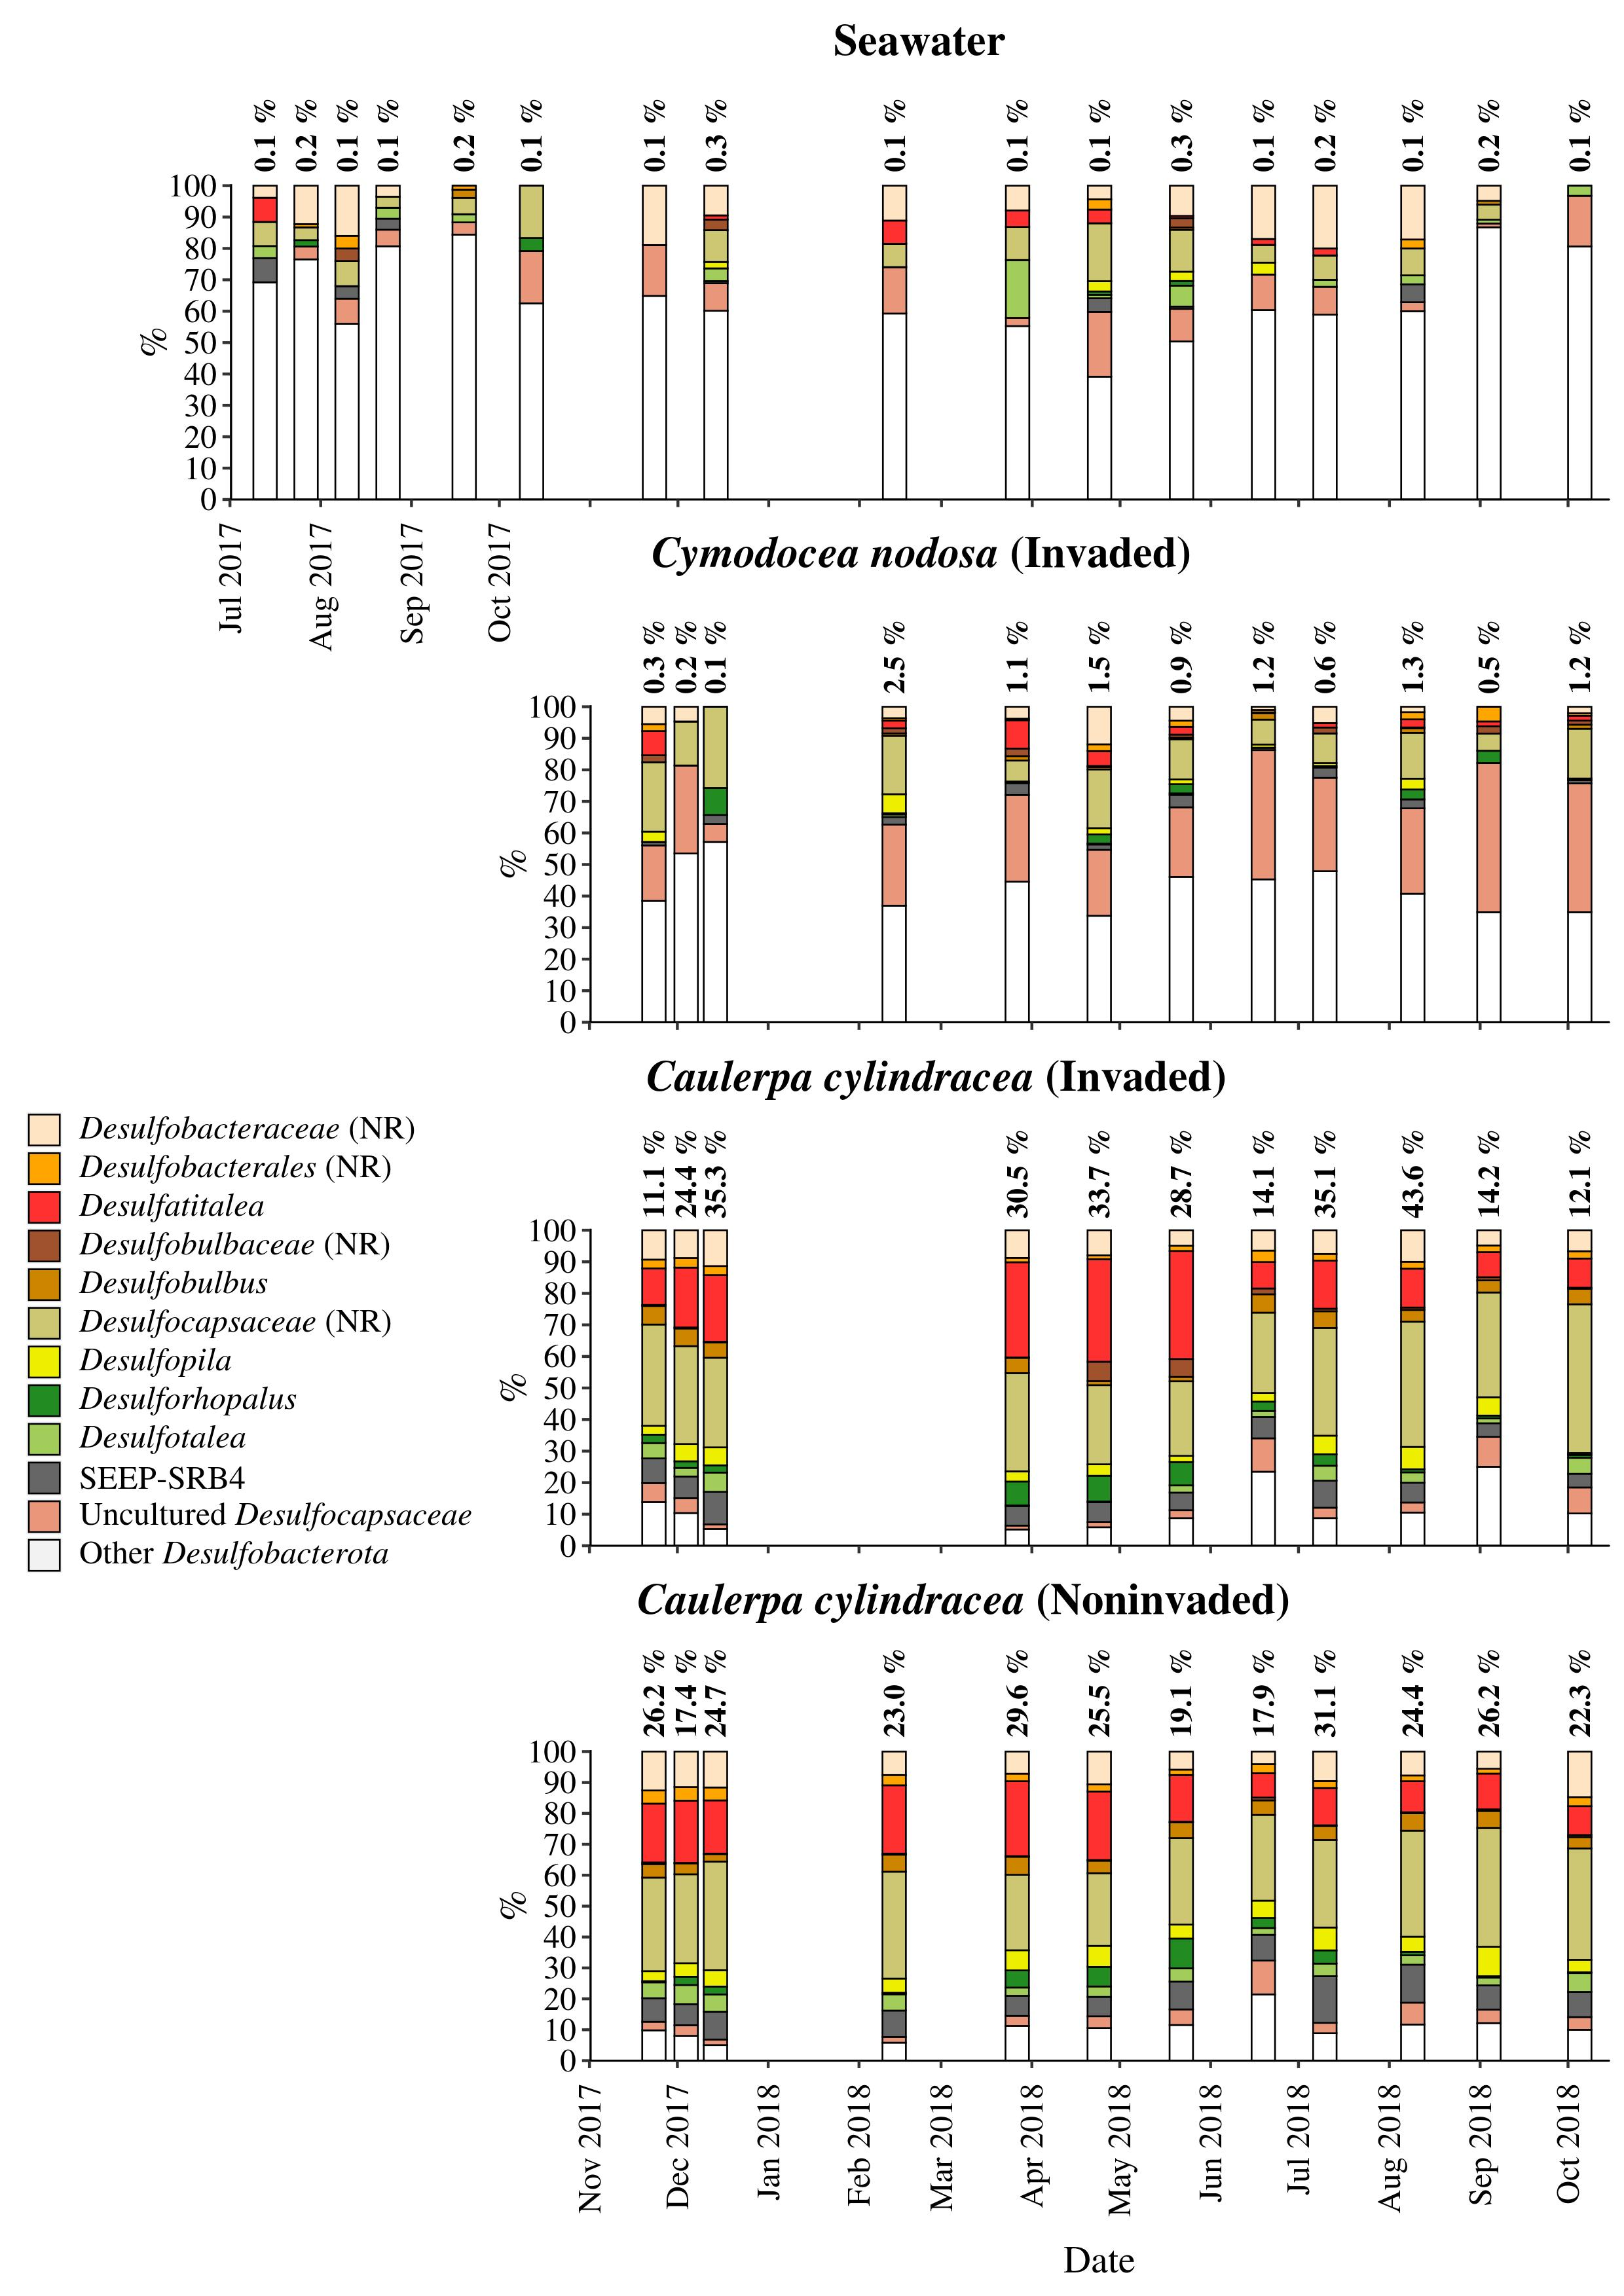
\includegraphics[width=0.85\linewidth]{../results/figures/desulfobacterota_bar_plot} 

}

\caption{Taxonomic classification and relative contribution of the most abundant sequences within the \textit{Desulfobacterota} on the surfaces of macrophytes (\textit{Cymodocea nodosa} [Invaded] and \textit{Caulerpa cylindracea} [Invaded and Noninvaded]) and in the surrounding seawater. The proprotion of sequences classified as \textit{Desulfobacterota} in the total bacterial and archaeal community is given above the corresponding bar. NR -- No Relative\label{desulfo}}\label{fig:unnamed-chunk-9}
\end{figure}


\end{document}
